%===============================================================================
% LaTeX sjabloon voor de bachelorproef toegepaste informatica aan HOGENT
% Meer info op https://github.com/HoGentTIN/latex-hogent-report
%===============================================================================

\documentclass[dutch,dit,thesis]{hogentreport}

% TODO:
% - If necessary, replace the option `dit`' with your own department!
%   Valid entries are dbo, dbt, dgz, dit, dlo, dog, dsa, soa
% - If you write your thesis in English (remark: only possible after getting
%   explicit approval!), remove the option "dutch," or replace with "english".

\usepackage{lipsum} % For blind text, can be removed after adding actual content

%% Pictures to include in the text can be put in the graphics/ folder
\graphicspath{{../graphics/}}

%% For source code highlighting, requires pygments to be installed
%% Compile with the -shell-escape flag!
%% \usepackage[chapter]{minted}
%% If you compile with the make_thesis.{bat,sh} script, use the following
%% import instead:
\usepackage[chapter]{minted}
\usemintedstyle{solarized-light}

%% Formatting for minted environments.
\setminted{%
    autogobble,
    frame=lines,
    breaklines,
    linenos,
    tabsize=4
}

%% Ensure the list of listings is in the table of contents
\renewcommand\listoflistingscaption{%
    \IfLanguageName{dutch}{Lijst van codefragmenten}{List of listings}
}
\renewcommand\listingscaption{%
    \IfLanguageName{dutch}{Codefragment}{Listing}
}
\renewcommand*\listoflistings{%
    \cleardoublepage\phantomsection\addcontentsline{toc}{chapter}{\listoflistingscaption}%
    \listof{listing}{\listoflistingscaption}%
}

% Other packages not already included can be imported here

%%---------- Document metadata -------------------------------------------------
% TODO: Replace this with your own information
\author{Goran Van Damme}
\supervisor{Mevr. S. Lambert}
\cosupervisor{Dhr. J. Khan}
\title%
    {Versterking van Bedrijfsnetwerkbeveiliging met behulp van Firewall toepassingen binnen VPK Packaging Group}
\academicyear{\advance\year by -1 \the\year--\advance\year by 1 \the\year}
\examperiod{1}
\degreesought{\IfLanguageName{dutch}{Professionele bachelor in de toegepaste informatica}{Bachelor of applied computer science}}
\partialthesis{false} %% To display 'in partial fulfilment'
%\institution{Internshipcompany BVBA.}

%% Add global exceptions to the hyphenation here
\hyphenation{back-slash}

%% The bibliography (style and settings are  found in hogentthesis.cls)
\addbibresource{bachproef.bib}            %% Bibliography file
\addbibresource{../voorstel/voorstel.bib} %% Bibliography research proposal
\defbibheading{bibempty}{}

%% Prevent empty pages for right-handed chapter starts in twoside mode
\renewcommand{\cleardoublepage}{\clearpage}

\renewcommand{\arraystretch}{1.2}

%% Content starts here.
\begin{document}

%---------- Front matter -------------------------------------------------------

\frontmatter

\hypersetup{pageanchor=false} %% Disable page numbering references
%% Render a Dutch outer title page if the main language is English
\IfLanguageName{english}{%
    %% If necessary, information can be changed here
    \degreesought{Professionele Bachelor toegepaste informatica}%
    \begin{otherlanguage}{dutch}%
       \maketitle%
    \end{otherlanguage}%
}{}

%% Generates title page content
\maketitle
\hypersetup{pageanchor=true}

%%=============================================================================
%% Voorwoord
%%=============================================================================

\chapter*{\IfLanguageName{dutch}{Woord vooraf}{Preface}}%
\label{ch:voorwoord}

%% TODO:
%% Het voorwoord is het enige deel van de bachelorproef waar je vanuit je
%% eigen standpunt (``ik-vorm'') mag schrijven. Je kan hier bv. motiveren
%% waarom jij het onderwerp wil bespreken.
%% Vergeet ook niet te bedanken wie je geholpen/gesteund/... heeft

\lipsum[1-2]
%%=============================================================================
%% Samenvatting
%%=============================================================================

% TODO: De "abstract" of samenvatting is een kernachtige (~ 1 blz. voor een
% thesis) synthese van het document.
%
% Een goede abstract biedt een kernachtig antwoord op volgende vragen:
%
% 1. Waarover gaat de bachelorproef?
% 2. Waarom heb je er over geschreven?
% 3. Hoe heb je het onderzoek uitgevoerd?
% 4. Wat waren de resultaten? Wat blijkt uit je onderzoek?
% 5. Wat betekenen je resultaten? Wat is de relevantie voor het werkveld?
%
% Daarom bestaat een abstract uit volgende componenten:
%
% - inleiding + kaderen thema
% - probleemstelling
% - (centrale) onderzoeksvraag
% - onderzoeksdoelstelling
% - methodologie
% - resultaten (beperk tot de belangrijkste, relevant voor de onderzoeksvraag)
% - conclusies, aanbevelingen, beperkingen
%
% LET OP! Een samenvatting is GEEN voorwoord!

%%---------- Nederlandse samenvatting -----------------------------------------
%
% TODO: Als je je bachelorproef in het Engels schrijft, moet je eerst een
% Nederlandse samenvatting invoegen. Haal daarvoor onderstaande code uit
% commentaar.
% Wie zijn bachelorproef in het Nederlands schrijft, kan dit negeren, de inhoud
% wordt niet in het document ingevoegd.

\IfLanguageName{english}{%
\selectlanguage{dutch}
\chapter*{Samenvatting}
\selectlanguage{english}
}{}

%%---------- Samenvatting -----------------------------------------------------
% De samenvatting in de hoofdtaal van het document

\chapter*{\IfLanguageName{dutch}{Samenvatting}{Abstract}}

Tegenwoordig is elke machine binnen een productiebedrijf op een of andere manier verbonden met het internet. Dit zorgt ervoor dat er veel efficiënter kan worden gewerkt, omdat verschillende delen van het productieproces beter op elkaar kunnen worden afgestemd. Dit kan enerzijds worden bereikt door gebruik te maken van ERP (Enterprise Resource Planning) systemen die communicatie tussen de verschillende actoren in de supply chain mogelijk maken.

Echter zal dit er ook voor zorgen dat de machines die verbonden zijn met het ICS (Industrial Control System) veel kwetsbaarder zijn voor cyberaanvallen van buitenaf. Dit is omdat er vaak gebruik wordt gemaakt van oude technologieën die een lange levensduur hebben. De aanvallers die controle over het ICS krijgen kunnen productieprocessen gijzelen en bedrijven dwingen tot het betalen van losgeld om de controle terug te krijgen. Dit kan leiden tot ernstige verstoringen in de productie en schade aan de reputatie van het bedrijf. Bovendien kan het stilleggen van belangrijke bedrijfsprocessen ook leiden tot vertragingen in de levering van producten, wat de hele supply chain kan beïnvloeden en resulteren in een grootschalige economische impact. Daarom is het interessant om een onderzoek te doen naar de meest effectieve firewalltoepassingen die het ICS van een productiebedrijf beter kunnen beschermen. 

Er worden verschillende methodes gebruikt, waaronder een uitgebreide literatuurstudie en analyse op basis van een casestudy. Ook zullen systeembeheerders hun kennis delen omtrent ICS aanvallen. Vorige attacks op de ICS zullen worden geanalyseerd en kunnen ons waardevolle inzichten geven over de aanvallen die het vaakst voorkomen op het ICS. Ook zal er gekeken worden naar de ICS aanvallen die over de hele wereld worden uitgevoerd. Hierdoor zullen we niet enkel nuttige data kunnen verzamelen over aanvallen die al gebeurd zouden zijn op het ICS van VPK, maar ook over aanvallen die mogelijks zouden kunnen gebeuren.

Hierdoor ontstaat er een overzicht van de manieren waarop productie bedrijven hun netwerken beveiligen en zal ook de firewall op een zo effectief mogelijke manier kunnen werken. Deze resultaten duiden niet alleen de effectiviteit van deze firewalltoepassingen aan, maar dienen ook voor het verbeteren van de algemene netwerkbeveiligingsstrategieën binnen het productiebedrijf.

Bovendien kan er besloten worden dat een een firewall een belangrijke rol blijft spelen in het beschermen van het ICS van het productiebedrijf tegen aanvallen van buitenaf. Er wordt nogmaals benadrukt hoe belangrijk firewalls zijn binnen het productiebedrijf die hightech werktuigen en systemen gebruiken die met elkaar verbonden zijn, enerzijds via het interne netwerk. En anderzijds door de verbinding met andere spelers in de supply chain zoals: leveranciers, klanten, ...


%---------- Inhoud, lijst figuren, ... -----------------------------------------

\tableofcontents

% In a list of figures, the complete caption will be included. To prevent this,
% ALWAYS add a short description in the caption!
%
%  \caption[short description]{elaborate description}
%
% If you do, only the short description will be used in the list of figures

\listoffigures

% If you included tables and/or source code listings, uncomment the appropriate
% lines.
\listoftables

\listoflistings

% Als je een lijst van afkortingen of termen wil toevoegen, dan hoort die
% hier thuis. Gebruik bijvoorbeeld de ``glossaries'' package.
% https://www.overleaf.com/learn/latex/Glossaries

%---------- Kern ---------------------------------------------------------------

\mainmatter{}

% De eerste hoofdstukken van een bachelorproef zijn meestal een inleiding op
% het onderwerp, literatuurstudie en verantwoording methodologie.
% Aarzel niet om een meer beschrijvende titel aan deze hoofdstukken te geven of
% om bijvoorbeeld de inleiding en/of stand van zaken over meerdere hoofdstukken
% te verspreiden!

%%=============================================================================
%% Inleiding
%%=============================================================================

\chapter{\IfLanguageName{dutch}{Inleiding}{Introduction}}%
\label{ch:inleiding}

\section{\IfLanguageName{dutch}{Probleemstelling}{Problem Statement}}%
\label{sec:probleemstelling}

Door de toenemende complexiteit en frequentie van cyberaanvallen is het steeds moeilijker en noodzakelijker voor bedrijven om zich te beschermen tegen deze dreigingen \autocite{saravanan2019}. Het is daarom uitermate belangrijk dat bepaalde organisaties zich hiertegen gaan wapenen met effectieve maatregelen op het vlak van cybersecurity. In dit onderzoek zal de focus liggen op het analyseren en evalueren van de huidige  firewalltoepassing binnen een bepaalde site van VPK en de impact op het beveiligen van het IT/OT netwerk van deze site.
Volgens \textcite{pan2017} is cybersecurity een hoge prioriteit bij veel bedrijven, vooral door het groeiende aantal machines en systemen die op één of andere manier verbonden zijn met het internet om te communiceren met onder meer ERP-systemen.  Volgens \textcite{Lin2017} worden ICS'en op grote schaal gebruikt in verschillende kritieke infrastructuren van onder andere de olie-, water- en elektriciteitsindustrie. In het verleden beschikten de meeste van deze ICS'en niet over authentificatie- en versleutelingsmechanismen zoals firewalls of Vitual Private Networks (VPN) , waardoor ze kwetsbaar waren voor aanvallen door hackers. Dit is een zwak punt in het netwerk van een productiebedrijf dat gebruik maakt van een ICS. Zonder een performante firewall zijn deze systemen zeer kwetsbaar voor allerhande cyberbedreigingen, met name deze op de ICS. Daarom is de keuze voor een geschikte firewalltoepassing belangrijk voor het beschermen van bedrijfsnetwerken tegen mogelijke aanvallen van buitenaf die schade kunnen aanrichten aan de industriële infrastructuur van het bedrijf. Door deze aanvallen kan tevens de dienstverlening van het bedrijf op grote schaal verstoord worden. Volgens \textcite{Nwanya2017} zou het bedrijf aanzienlijk grote verliezen kunnen lijden door de stilstand van de productie. Het doel van dit onderzoek is dan ook om systeembeheerders en IT-professionals binnen VPK gerichtere informatie te geven over welke firewall-opstelling ze het best gebruiken binnen de productiesite. Deze informatie helpt hen bij het uitkiezen van de meest effectieve firewall, zodat zij de beveiliging van hun IT-infrastructuur kunnen waarborgen en de continue werking van de productie kunnen garanderen. Hierdoor kunnen de bevindingen van dit onderzoek direct worden toegepast in relevante cases binnen VPK.

\section{\IfLanguageName{dutch}{Onderzoeksvraag}{Research question}}%
\label{sec:onderzoeksvraag}

Daarom zal dit onderzoek de uitdaging aankaarten die VPK heeft bij het kiezen van de juiste firewalltoepassing die haar infrastructuur zal beschermen tegen aanvallen op het ICS. Dit kan verschillen van bedrijf tot bedrijf. Daarom is een gepaste onderzoeksvraag voor deze bachelorproef: ``\texttt{Welke firewalltoepassingen zal het beste ICS-aanvallen tegengaan binnen VPK Packaging Group?}''

\begin{itemize}
    \item ``\texttt{Welke zwaktes in de huidige IT/OT architectuur maken VPK kwetsbaar voor ICS-aanvallen?}''
    \item ``\texttt{Welke soorten firewall systemen worden er momenteel gebruikt binnen VPK?}''
    \item ``\texttt{Welke kosten en onderhoudsvereisten zijn verbonden aan de implementatie van een nieuwe firewall?}''
    \item ``\texttt{Hoe kan de gekozen firewalltoepassing optimaal worden geïmplementeerd en geconfigureerd binnen de bestaande IT/OT-infrastructuur van VPK Packaging Group?}''
    \item ``\texttt{Welke specifieke problemen zijn er met de huidige firewalls opstelling?}''
    \item ``\texttt{Welke verschillende firewall settings kunnen worden aangepast om de beveiliging nog effectiever te maken.}``
    \end{itemize}

\section{\IfLanguageName{dutch}{Onderzoeksdoelstelling}{Research objective}}%
\label{sec:onderzoeksdoelstelling}

Dit onderzoek zal beperkt blijven tot het beveiligen van de ICS van het bedrijf. Mogelijks zullen door aanpassingen aan de infrastructuur voor de optimalisatie van de bescherming van de ICS ook andere delen van het netwerk beter beschermd zijn. Echter is dit niet het hoofddoel. Het doel van dit onderzoek is ook om betere inzichten te krijgen in de trend van de verschillende soorten firewalltoepassingen en de verschillende use cases in de praktijk. Dit doel zal bereikt worden door een uitgebreide literatuurstudie en het analyseren van deze casestudy binnen een specifiek productiebedrijf. En daarna deze kennis toe te passen om het ICS van het bedrijf beter te beschermen tegen aanvallen. Dit alles zal worden samengevat in een rapport waarin een groot aantal aanbevelingen staan voor leden van het cybersecurityteam binnen het productiebedrijf. Hierdoor zullen zij beter in staat zijn om hun infrastructuur te beschermen tegen ICS-cyberaanvallen van buitenaf. Ook zullen zij bedreigingen beter kunnen identificeren, en hierdoor veilige en effectieve firewalltoepassingen kunnen implementeren. Daardoor zal het doel van deze bachelorproef ook bereikt zijn en zal VPK beter beschermd zijn tegen de steeds gevaarlijkere en grootschaligere ICS-dreigingen. Dit zorgt ervoor dat de downtime van machines en de integriteit van data binnen het bedrijf steeds gewaarborgd blijven. Deze onderzoeksdoelstelling is specifiek, meetbaar, acceptabel, relevant en tijdsgebonden (SMART) en zal daardoor resulteren in een stevige set van aanbevelingen voor betere cybersecurity practices.

\section{\IfLanguageName{dutch}{Opzet van deze bachelorproef}{Structure of this bachelor thesis}}%
\label{sec:opzet-bachelorproef}

% Het is gebruikelijk aan het einde van de inleiding een overzicht te
% geven van de opbouw van de rest van de tekst. Deze sectie bevat al een aanzet
% die je kan aanvullen/aanpassen in functie van je eigen tekst.

De rest van deze bachelorproef is als volgt opgebouwd:

In Hoofdstuk~\ref{ch:stand-van-zaken} wordt een overzicht gegeven van de stand van zaken binnen het onderzoeksdomein, op basis van een literatuurstudie.

In Hoofdstuk~\ref{ch:methodologie} wordt de methodologie toegelicht en worden de gebruikte onderzoekstechnieken besproken om een antwoord te kunnen formuleren op de onderzoeksvragen.

In Hoofdstuk~\ref{ch:onderzoek} zullen er verschillende analyses worden opgesteld om te gebruiken bij het maken van een doorwogen keuze omtrent de beste cybersecurity oplossing voor de productie.

In Hoofdstuk~\ref{ch:configFW} worden de configuratie van een firewall binnen VPK beter toegelicht en de keuzes die gemaakt zijn worden in detail beschreven.

In Hoofdstuk~\ref{ch:conclusie} tenslotte, wordt de conclusie gegeven en een antwoord geformuleerd op de onderzoeksvragen. Daarbij wordt ook een aanzet gegeven voor toekomstig onderzoek binnen dit domein.
\chapter{\IfLanguageName{dutch}{Stand van zaken}{State of the art}}%
\label{ch:stand-van-zaken}

\section{Inleiding tot industriele netwerkbeveiliging.}

\subsection{Wat is een firewall}
Volgens \textcite{ciscoFW2025} is de definitie van een firewall `Een netwerkbeveiligingsapparaat dat een vertrouwd intern netwerk scheidt van een extern netwerk dat als onbetrouwbaar wordt beschouwd, zoals bijvoorbeeld het internet.` Het regelt inkomend en uitgaand netwerkverkeer op basis van vooraf ingestelde beveiligingsregels. Firewalls zijn van het grootste belang bij het afschermen van netwerken tegen ongeautoriseerde toegang, schadelijke activiteiten en potentiële bedreigingen.
Op deze manier kan de beheerder van de firewall kunnen beslissen welk verkeer er in en uit zijn netwerk gaat. Hierdoor kan men het interne netwerk beschermen tegen dreigingen van buitenaf.



Een firewall kan bestaan in verschillende vormen, binnen deze zelfde bron van Cisco worden er een groot aantal firewalls doorlopen. Een aantal bekende en veelgebruikte firewalls zijn de statefull inspection firewalls, packet filtering firewall's  en NGFW's.
 
Packet filtering firewalls zullen elk pakket onafhankelijk evalueren, zonder verbindingen bij te houden. Elk pakket zal individueel worden beoordeelt aan de hand van de door de beheerder gedefinieerde regels. Dit vereist vaak aparte regels voor zowel het uitgaand (outbound) als inkomend (inbound) verkeer. De mogelijkheid om te specifieren of een filter inbound of outbound is geeft je grotere controle over waar de router verschijnt in het filterschema , en is zeer handig voor het filteren op routers met meer dan twee interfaces. Als bepaalde pakketten gedropt kunnen worden door een inbound filter op een interface, dan moeten die pakketten niet vermeld te worden in de outbound filters op alle andere interfaces.. Men zal dan filters kunnen gaan toepassen voor bepaalde parameters van het pakket zoals source IP adres, destination IP adres en poortnummer maar ook aan de hand van het gebruikte IP protocol. Hoewel deze 'stateless firewalls' vandaag de dag minder vaak gebruikt worden, zijn ze nog steeds aanwezig in sommige netwerkapparatuur, vaak zijn dit switches of routers. Het grootste verschil tussen deze statefull en stateless firewalls is dat de stateless firewalls zoals de naam het zegt geen staten van verbindingen zullen gaan bijhouden, zij zullen regels toepassen op alle pakketten zonder rekening te houden met hun context. \autocite{goel2014}

Volgens \textcite{paloAltoSF2025} zou men dit probleem kunnen oplossen door gebruik te maken van packet filteren firewalls, deze firewalls worden ook wel 'statefull firewalls' genoemd. In tegenstelling tot stateless inspectie die elk pakket afzonderlijk behandelt, ziet de statefull firewall het netwerkverkeer als een continue stroom. Dit doet hij onder andere door te kijken naar de 'three way handshake'. Dit maakt het mogelijk om patronen te detecteren die wijzen op potentiële bedreigingen. Stateful inspection analyseert de header van het pakket om te bepalen of het deel uitmaakt van een bestaande conversatie. Als een pakket niet overeenkomt met een bestaande verbinding, dan wordt het geëvalueerd aan de hand van de vooraf beschreven firewallregels om te beslissen of het doorgelaten moet worden. Volgens Palo Alto zouden statefull firewalls actieve verbindingen intelligenter beheren, waardoor de netwerkbronnen efficiënter gebruikt kunnen worden. Pakketten van vertrouwde verbindingen hoeven op deze manier niet voortdurend opnieuw geëvalueerd te worden. Dit zorgt ervoor dat de verwerkingslast wordt verlaagt en de doorvoersnelheid wordt gemaximaliseerd. 

Vandaag de dag wordt er als maar meer gebruik gemaakt van Next Generation Firewalls (NGFW’s) die diepe packet inspection uitvoeren en op basis hiervan zullen beslissen of een packet wordt geblokkeerd of niet. Sedert 2020 maken deze NGFW’s ook gebruik van Artificiële Intelligentie (AI). \autocite{Ahmadi2023}. Firewalls die gebruik maken van AI genereren beveiligingsmaatregelen en dwingen deze af op basis van het continue netwerkverkeer waardoor de blootstelling aan nieuwe bedreigingen aanzienlijk wordt verminderd. \autocite{PaloAltoFW2024}

Ondanks de snelle evolutie van firewalls blijft een groot struikelblok bij het toepassen hiervan de complexiteit van bedrijfsnetwerken. Volgens \textcite{Bringhenti2023} wordt het configureren van security functies typisch nog steeds manueel gedaan. Maar omdat moderne netwerken zodanig complex en dynamisch zijn, is de manuele configuratie hiervan niet haalbaar. Dit zorgt ervoor dat het kiezen van een gepaste firewall niet alleen draait om de manier waarop mogelijke threats worden afgehandeld, maar ook de manier waarop de automatisatie en configuratie zullen kunnen worden toegepast.



\subsection{Evolutie van firewalls}
Firewalls bestaan al sinds de jaren’ 80, toendertijd deden firewalls slechts enkel aan basic packet filtering. Sindsdien zijn firewalls steeds blijven evolueren, enerzijds door de groeiende digitalisering en anderzijds door de grotere cyberdreigingen tegen industriële infrastructuur van productiebedrijven \autocite{Wusteney2021}. 
Vandaag de dag wordt er gebruik gemaakt van Next Generation Firewalls (NGFW’s) die diepe packet inspection uitvoeren en op basis hiervan beslissen of een pakket wordt geblokkeerd of niet. Sedert 2020 maken deze NGFW’s ook gebruik van Kunstmatige Intelligentie (AI) \textcite{Ahmadi2023}. Firewalls die gebruik maken van AI genereren beveiligingsmaatregelen en dwingen deze af op basis van het continue netwerkverkeer, waardoor de blootstelling aan nieuwe bedreigingen aanzienlijk wordt verminderd \textcite{PaloAltoFW2024}.

  
\subsection{Belang van cybersecurity in een productieomgeving}

De golfkartonindustrie is sterk afhankelijk van onderling verbonden systemen, waardoor cybersecurity essentieel is. OT zal belangrijke productieprocessen gaan beheren die grondstoffen omzetten in nauwkeurige verpakkingen van hoge kwaliteit, zoals het snijden en printen van golfkarton en zorgt zo voor efficiëntie en kwaliteit. Ook zal real-time bewaking binnen deze systemen de productkwaliteit op peil houden en zo verspilling minimaliseren. Door het monitoren van de machines zal er efficiënter kunnen worden ingespeeld op het onderhoud waardoor deze machines een langere levensduur zullen hebben. Naarmate OT-systemen en CPS meer met elkaar verbonden raken, is het van cruciaal belang om ze te beveiligen tegen cyberbedreigingen. Een inbreuk kan de productie verstoren, de kwaliteit in gevaar brengen en gevoelige informatie blootleggen. In de huidige industrie beschermt robuuste OT beveiliging zowel de productie-integriteit als de bedrijfscontinuïteit. \autocite{fefco2025}

Deze toename in connectiviteit tussen systemen zorgt er niet alleen voor dat nieuwe eisen nodig zijn op het vlak van cybersecurity, maar heeft ook een impact op de bescherming van het ICS zeker als we weten dat de beveiliging van het ICS lange tijd als minder belangrijk werd beschouwd. Vaak werd er gewerkt met "security through obscurity" wat betekent dat systemen werden beschermd door informatie geheim te houden in plaats van echte beveiligingsmaatregelen te implementeren. Dit werkte redelijk goed voor oudere systemen, omdat ze enkel in contact stonden met apparaten vanop het eigen netwerk en amper verbonden waren met apparaten buiten hun netwerk. Bij de derde en tevens ook nieuwste generatie ICS is deze aanpak echter veel minder effectief. Moderne systemen maken gebruik van open technologieën om te communiceren met andere niet-ICS netwerken, waaronder het internet. Hierdoor is de beveiliging door onduidelijkheid niet langer voldoende, omdat aanvallers steeds beter bekend zijn met de gebruikte technologieën en kwetsbaarheden makkelijker kunnen vinden. \autocite{knowles2015}

Ondanks de snelle evolutie van firewalls blijft een groot struikelblok bij het toepassen hiervan de complexiteit van bedrijfsnetwerken. Volgens Bringhenti e.a. (2023) wordt het configureren van security functies typisch nog steeds manueel gedaan. Maar omdat moderne netwerken zodanig complex en dynamisch zijn, is de manuele configuratie hiervan niet haalbaar. Het kiezen van een gepaste firewall draait niet alleen om hoe mogelijke bedreigingen worden afgehandeld, maar ook om hoe automatisatie en configuratie kunnen worden toegepast.


\subsection{Verschil tussen IT en OT infrastructuur en beveiliging}

OT omvat een breed scala aan programmeerbare systemen en apparaten die direct of indirect in interactie zullen gaan met de fysieke omgeving. Veelvoorkomende OT-toepassingen zijn Supervisory Control and Data Acquisition (SCADA) voor grootschalige procesmonitoring, Programmable Logic Controllers (PLC) voor de besturing van machines en productielijnen. Daarnaast omvat OT ook de Industrial Internet of Things (IIoT) voor het verbinden van industriële apparaten en sensoren. OT kan worden ingezet voor het monitoren, besturen en automatiseren van industriële processen, transport en energiebeheer. Deze systemen bestaan uit verschillende onderdelen met elk eigen functies. Zoals mechanische, elektrische, hydraulische en pneumatische onderdelen, die samenwerken om bepaalde doelstelling te behalen. \autocite{Stouffer2023}.

Hoewel OT-systemen traditioneel geïsoleerd waren, worden ze steeds vaker gekoppeld aan IT-netwerken, wat voordelen biedt op het gebied van efficiëntie en gegevensanalyse, maar ook nieuwe beveiligingsrisico’s met zich meebrengt. Daarom is een robuuste beveiligingsarchitectuur essentieel voor het waarborgen van de betrouwbaarheid en integriteit van OT-systemen. \autocite{Stouffer2023}.

\section{Firewall technologieen en hun rol in de ICS beveiliging}

\subsection{Sophos en Palo Alto firewalls binnen het VPK netwerk.}
Om het onderzoek in deze bachelorproef goed te begrijpen, is een basiskennis van tweefirewall merken essentieel: Sophos en Palo Alto. Sophos firewalls staan erom bekend dat ze zeer gebruiksvriedelijke userinterfaces en geintegreerde beveiligingsoplossingen hebben. Ze bieden een breed scala aan functies aan waaronder deep packet inspection (DPI), intrusion prevention system (IPS), geavanceerde dreigingsanalyse en synchronisatie met andere Sophos producten via Synchronized Security. \autocite{Phipps2024}

Palo Alto firewalltoepassingen onderscheiden zich dan weer door hun geavanceerde applicatie- en identiteitsgebaseerde beveiligingsfuncties. Daarnaast biedt Palo Alto ook krachtige IPS en IDS toepassingen die het bedrijf kunnen beschermen tegen malware en andere cyberdreigingen. Palo Alto maakt geeft ook de mogelijkheid om gebruik te maken van hun cloud based beheerplatform met de naam Strata Cloud. Deze beveiligingssuite zorgt ervoor dat bedrijven hun infrastructuur kunnen beschermen ongeacht of ze zich on-premises,in de cloud of in hybride omgevingen bevinden. \autocite{shread2023}

Er zijn wel degelijk een aantal grote verschillen tussen deze twee firewall vendors. Sophos firewalls zijn bijzonder gebruiksvriendelijk, met een eenvoudig beheerplatform via Sophos Central, wat ideaal is voor kleinere bedrijven. Palo Alto biedt meer geavanceerde functionaliteiten, maar vereist een diepere technische kennis voor configuratie en beheer van de firewall. Beide firewalls hebben een cloud based beheerplatform. Echter zal Sophos Central zich meer richten op eenvoudig beheer, terwijl Palo Alto Strata een uitgebreider platform is voor hybride en multi-cloud omgevingen. \autocite{paloGuard2025} 

Echter wil dit niet direct zeggen dat de ene firewall voor alle use-cases beter is dan de anderefirewall. Het kiezen van het juiste merk van firewall hangt heel erg af van de schaal van hetnetwerk waarin deze zich zal bevinden. Ook de ervaring van het netwerkteam dat de infrastructuur beheerd kan een grote rol spelen in de keuze. Heeft het team al eerder gewerkt met firewalls van een bepaalde vendor? Bestaat het team uit ervaren medewerkers of eerder uit junior profielen? Dit zijn allemaal zaken die je in je achterhoofd moet houden bij het kiezen van een firewall toepassing.



\subsection{Segmentatie als beveiligingstoepassing}
Firewalls worden gebruikt door organisaties om interne infrastructuur te beschermen tegen ongeautoriseerde toegang door data te inspecteren en bepaalde beveiligingsmaatregels toe te passen. Echter zal een firewall ook kunnen worden gebruikt voor het verdelen van het netwerk in meerdere delen die elk verschillende beveiligingseisen hebben. Een multinational zoals VPK heeft honderden firewalls waardoor de configuratie en locatie van de firewall’s in het netwerk cruciaal zijn. Om deze honderden firewalls correct te segmenteren heeft men een plan nodig die op iedere firewall zal worden uitgevoerd. Op deze manier zal iedere firewall op dezelfde manier geconfigureerd zijn. En wordt de kans op eigenaardigheden beperkt. Ook zal het beheren van de firewalls na de installatie een stuk vlotter gaan als alle firewalls in een uniforme manier zijn opgezet.
Twee veelgebruikte strategieën bij het beveiligen van een netwerk zijn gelaagde beveiliging en segmentatie. Gelaagde beveiliging, ook wel gekend als Defence in Depth (DD), zorgt ervoor dat een netwerk meerdere beveiligingslagen bevat. Iedere laag heeft apparte beveiligingsmaatregelen. Dit zorgt ervoor dat als een attacker door een van de lagen penetreert, de andere lagen nog steeds het netwerk zullen beveiligen. \autocite{FortinetDE2025} Bij netwerksegmentatie wordt de infrastructuur ingedeeld in verschillende zones, elke zone is beschermd door een of meerdere firewalls die afgstemd zijn op specifieke beveiligingseisen van die welbepaalde zone. Echter zijn er geen duidelijke richtlijnen aanwezig om segmentatie op een efficiente manier aan te pakken. Hierdoor kan dit soms uitdagend zijn. \autocite{Mhaskar2021}
Een andere manier van segmentatie is het gebruiken van een DMZ (Demilitarized Zone). Dit is een soort van subnetwerk dat zich tussen het interne LAN en het WAN bevindt. In dit netwerk zullen publiekgerichte services beschikbaar zijn. Enkele voorbeelden van services die vaak in de DMZ gehost zijn, zijn de DNS server, mailserver en webserver. \autocite{Patel2020}



\section{ICS architectuur binnen een industriële omgeving}

\subsection{Doel van SWOT en RASCI binnen een vergelijkende studie}
SWOT staat voor strenghts, weakneses, opportunities and threats en is een tool die wordt gebruikt om belangrijke interne en externe factoren te begrijpen die een organisatie of project beïnvloeden. SWOT werd ontwikkeld door Albert Humphrey in de jaren '60 en '70. Een SWOT analyse helpt bij het maken van strategische keuzes door het identificeren van sterke en zwakke punten, maar ook door externe kansen en bedreigingen. Hoewel het maken van een SWOT analyse eenvoudig lijkt, vereist een goede SWOT analyse tijd, massaal veel tijd en middelen. dit komt omdat het vinden van de juiste factoren niet altijd eenvoudig of straight forward is. Onjuiste aannames kunnen leiden tot vertragingen in strategische keuzes.\autocite{cipd2025}

SWOT analyses hebben verschillende voor en nadelen. De grootste voordelen die een SWOT analyse biedt is de graad waarin het in een bedrijf kan worden toegepast. Het kan gebruikt worden voor het beoordelen van een kleinschalig project, maar evengoed voor het beoordelen van de volledige bedrijfsstrategie. Ook is het makkelijk om op te stellen. Je hebt geen uitgebreide wiskundige kennis nodig voor het opstellen van het diagram. Echter zijn er ook een aantal nadelen aan verbonden. Zo kan het zijn dat een SWOT analyse wordt opgesteld op basis van assumpties en vooroordelen en niet op basis van feiten. Een analyse die op deze manier wordt gedaan, is in de praktijk echter niet zo waardevol. \autocite{sarsby2012}


Volgens \textcite{putman2024} is het RASCI-model een tool die wordt gebruikt om rollen en verantwoordelijkheden binnen een project of organisatie te verduidelijken. Het staat voor responsible, accountable, supporting, consulted en informed. Het model helpt bij het structureren van verschillende taken en bevoegdheden. Het model wordt vaak gebruikt binnen het projectmanagement om onduidelijkheden omtrent bevoegdheden te voorkomen. Binnen een grootschalige industriele omgeving zoals die van VPK kan RASCI bijdragen aan een vlotte en efficiente samenwerking tussen IT en OT teams door duidelijk vast te leggen wie verantwoordelijk is voor implementatie, wie eindverantwoordelijk is, wie ondersteuning biedt, wie geraadpleegd moet worden en wie op de hoogte gehouden moet worden. Vaak wordt er echter gebruik gemaakt van het RACI model, hierbij zal de supporting role van het RASCI model worden weggelaten. Deze methode wordt vooral gebruikt binnen organisaties met een minder complexe samenwerkingsstructuur. \autocite{harkhoe2025}





\subsection{Overzicht van de verschillende ICS componenten}
Binnen eender welke productiesite van VPK zal je in aanraking komen met de verschillende componenten die deel uitmaken van de OT omgeving. Daarom kan het zeker geen kwaad om te weten uit welke componenten de algemene VPK productie-site is opgebouwd. 

Omdat de meeste fabrieken vandaag de dag nog niet 100 \% autonoom kunnen werken zonder tussenkomt van een operator die de machine bestuurd zal er steeds nood zijn aan een bepaalde manier om input van de operator door te geven aan de machine. Dit zal vaak gebeuren op basis van een HMI (Human-Machine Interface). 
Volgens \textcite{Nist2025} is een HMI De hardware of software waarmee een operator communiceert met een controller. Een HMI kan variëren van een fysiek bedieningspaneel met knoppen en indicatielampjes tot een industriële pc met een grafisch kleurenscherm waarop speciale HMI-software draait. De operatoren kan via deze interface bepaalde bedieningen uitvoeren op de machine. In andere woorden zal een HMI er voor zorgen dat bepaalde configuraties die de operator wil maken op een efficiente en duidelijke manier voor de operator worden doorgevoerd naar de machine. 
Nu zal de HMI niet enkel worden gebruikt voor het invoeren van data voor een operator, hij kan ook worden gebruikt voor het tonen van belangerijke informatie van de machine aan de operator zoals grafieken, diagrammen en digitale dashboards. \autocite{Inductive2025}
Volgens \textcite{Copadata2025} zou je technisch gezien de term HMI kunnen toepassen op elk scherm dat iemand gebruikt voor interactie met een apparaat, maar de term wordt meestal gebruikt om schermen te beschrijven die in industriële omgevingen worden gebruikt. 
Een PLC (Programmable Logic Controller) is een apparaat dat cruciaal is binnen eender welke productiesite. De PLC is in staat om op basis van bepaalde invoerapparaten zoals sensoren beslissingen te maken aan de hand van “ladder logical”. Deze beslissingen triggeren dan weer acties die zullen worden ondernomen door aangesloten output apparaten zoals relais, LED’s, pneumatica en aandrijvingen \autocite{unitronics2025}.
Vaak zal de besturing van de PLC gebeuren aan de hand van een HMI, echter zal de operator van de HMI geen daadwerkelijke code moeten schrijven, maar kan hij bepaalde data zien of handelingen uitvoeren via speciale software die beschikbaar is op de grafische gebruikersinterface van de HMI. 
Echter is het verzamelen van data aan de hand van PLC’s en andere slimme industriele sensoren niet genoeg, men moet deze dat kunnen omvormen naar nuttige informatie die gebruikt kan worden om het gebruiksgemak en de efficientie te verhogen. Een manier om dit te doen is door gebruik te maken van SCADA-systemen. 
Deze systemen zullen gebruik maken van HMI’s om de verkregen data van de verschillende sensoren omvormen, om op hoog niveau controle, beheer en toezicht te houden op industriële processen. SCADA netwerken zijn cruciaal voor industriële activiteiten, maar bestaan uit verouderde hardware en software die gemakkelijk gehackt kunnen worden, waardoor SCADA-beveiliging steeds belangrijker wordt.\autocite{FortinetSC2025}. SCADA moet dus eigenlijk niet gezien worden als een onderdeel van het ICS maar eerder als een type van ICS. 
Volgens \textcite{Mhaskar2021} is ICS een verzamelnaam voor verschillende soorten apparaten, systemen, netwerken en besturingen die worden gebruikt om industriële processen te bedienen en/of te automatiseren. Wat SCADA in deze context zal doen is het beheren en samenbrengen van allerlei databronnen om deze te verwerken.


\subsection{Zones, conduits en Purdue model voor ICS netwerken.}
Security zones zijn groepen systemen en componenten die functioneel, logisch of fysiek bij elkaar horen en dezelfde beveiligingseisen delen. Denk bijvoorbeeld aan een zone met alle PLC’s binnen de productie van een site of een zone met alle HMI’s en camerafeeds in een controlekamer. Door systemen op deze manier te groeperen, wordt het eenvoudiger om gerichte beveiligingsmaatregelen toe te passen en risico’s beheersbaar te houden. De communicatie tussen deze zones verloopt via conduits, dit zijn de verbindingslijnen tussen verschillende zones. Dit kunnen fysieke of logische verbindingen zijn, zoals ethernetnetwerken,fiber kabels of VPN-tunnels . Conduits bepalen welke informatie tussen zones mag worden uitgewisseld en zorgen ervoor dat alleen geautoriseerde communicatie tussen twee apparaten zal plaatsvinden. Op deze manier wordt de ongewenste toegang tot verschillende systemen zo minimaal mogelijk gehouden. Zodat de potentiele aanval niet zomaar van de ene naar de andere zone kan overslaan. \autocite{Dragos2023}
Je mag het ontwerpen van zones en conduits niet zien als een gesloten process. Na verloop van tijd veranderen er zaken in de architectuur waardoor de zones en conduits mogelijk niet meer optimaal zijn verdeeld. Daarom is het belangrijk om continue dit process the reevalueren en tijdig aanpassingen uit te voeren. Het is de bedoeling dat je voortdurend verbeteringen aanbrengt, waarbij de risicos op aanvallen worden verlaagd. \autocite{Incibe2018}
Een vaak gebruikt model waarbij we het netwerk zullen opdelen in verschillende zones is het Purdue model. Dit is een model dat ontwikkeld is aan de Purdue Universiteit in de Verenigde Staten begin jaren `90. Volgens \textcite{Mathezer2021}heeft het model als doel om best practices te definiëren voor de relatie tussen industriële besturingssystemen en bedrijfsnetwerken of met andere woorden tussen IT en OT. 
Ondanks de vele dynamische cyberdreigingen in het huidige OT landschap blijft het Purdue model een hoeksteen voor het beveiligen van het OT netwerk. Het grote voordeel aan dit model is dat de schaalbaarheid het geschikt maakt voor bedrijven met een grotere omvang. Omdanks de wat oudere leeftijd van dit model en de steeds meer geavanceerdere aanvallen op het OT netwerk blijven de kernprincipes zoals segmentatie, in-depth defence en risicobeheer essentieel voor het beperken van cyberrisico's in industriële omgevingen.

\subsection{Oplossingen voor de complexiteit van een firewall implementatie.}

Ondanks de snelle evolutie van firewalls blijft een groot struikelblok bij het toepassen hiervan de complexiteit van bedrijfsnetwerken. Volgens \textcite{Bringhenti2023} wordt het configureren van security functies typisch nog steeds manueel gedaan. Maar omdat moderne netwerken zodanig complex en dynamisch zijn, is de manuele configuratie hiervan niet haalbaar. Het kiezen van een gepaste firewall draait niet alleen om hoe mogelijke bedreigingen worden afhandelen, maar ook om hoe automatisatie en configuratie kunnen worden toegepast.

Er is een manier om de complexiteit van een groot bedrijfsnetwerk te verminderen door het toepassen van netwerksegmentatie \autocite{Bringhenti2023}. Hierdoor wordt het schrijven van veiligheidsmaatregelen beheersbaar en kunnen er robuuste security policies worden opgesteld voor het netwerk. Palo Alto Networks is een van de marktleiders op het vlak van cybersecurity-toepassingen, waaronder NGFW’s, cloud-based security services, advanced endpoint protection en threat intelligence \autocite{TechnicalWhitepaper2014}.

Palo Alto heeft bijvoorbeeld een cloud-based malware protection engine genaamd WildFire. WildFire is een Intrusion Detection System (IDS) die bestanden, die als mogelijke dreiging worden gecategoriseerd, uitvoert in een sandbox omgeving. Hier worden de dreigingen geanalyseerd met behulp van machine learning algoritmes die gedrag en patronen detecteren die indicatief zijn voor kwaadaardige activiteit \autocite{PaloAltoWF2024}.




\section{verschillende dreigingen op het ICS}

\subsection{Specifieke ICS aanvallen}

De laatste jaren is het cyberbeveiligingsbewustzijn sterk gegroeid, dit komt onder andere door verschillende grootschalige cyberaanvallen die de afgelopen jaren plaatsvonden. Een van de eerste grootschalige aanvallen die het gedachtegoed rond cybersecurity heeft veranderd is het Stuxnet-incident in 2010, dat gericht was op de Iraanse kerncentrale Natanz en ongeveer 25\% van de centrifuges voor uraniumverrijking beschadigde. \autocite{Zetter2014}. 

Ook viel de Shamoon-malware in 2012 het Saudische oliebedrijf Saudi Aramco en het Qatarese aardgasbedrijf RasGas aan, waarbij data werd vernietigd en geïnfecteerde systemen onbruikbaar werden \autocite{Hemsley2018}.
In diezelfde bron wordt er ook gesproken over een van de eerste publieke bekende cyberaanvallen op het elektriciteitsnet, een aanval op een Oekraïense energiebedrijf in 2015 ervoor zorgde dat bijna een kwart miljoen mensen zonder elektriciteit kwamen te zitten.

Echter zijn niet alle cyberaanvallen succesvol, volgens \textcite{Margolin2021} zou februari 2021 de Bruce T. Haddock Water Treatment Plant in Florida gehackt zijn door cybercriminelen. Die plant gebruikte een verouderd besturingssysteem waardoor de hacker toegang kreeg tot het computersysteem en de chemische niveaus van de watervoorziening kon wijzigen. De aanval werd ontdekt nog voordat er grote schade kon worden aangebracht.



Volgens \textcite{Morgan2024} werd de schade die cyberattacks aangericht zouden hebben in 2024 geschat op 9,5 biljoen dollar. Nu is de schatting voor de schade die ze zullen aanrichten in 2025 geschat op 10,5 biljoen dollar, dat is een steiging van maar liefst 15\% . Dit maakt dat cybercriminaliteit de op twee na grootste economie ter wereld is, na de VS en China.

\subsection{Insider threats vs Outsider threats}
Bij het opstellen van een cybersecurity plan wordt er vaak rekening gehouden met twee verschillende soorten threats. Aan de ene kant heb je de insider threats. Dit zijn dreigingen die worden veroorzaak door insiders. Volgens \textcite{Cisa2025} is een insider een persoon die geautoriseerde toegang heeft of had tot kennis van de middelen van een organisatie, zoals personeelsbestanden, faciliteiten, informatie, apparatuur, netwerken en systemen. In diezelfde bron worden een aantal voorbeelden gegeven van insider threats: Een persoon die de organisatie vertrouwt, inclusief werknemers, leden van de organisatie en personen aan wie de organisatie gevoelige informatie en toegang heeft gegeven. In dit geval gaat het over een werknemer die legitieme toegang heeft tot gevoelige informatie over het bedrijf.

Alhoewel dat de insider threats niet zo vaak aan bod komen in het nieuws brengen ze gemiddeld wel het meeste schade toe aan de organisatie. Volgens \textcite{ibm2024} leidden aanvallen van kwaadwillende insiders tot de hoogste kosten, gemiddeld 4,99 miljoen dollar. Andere dure aanvalsvectoren waren de compromisen van zakelijke e-mail, phishing, sociale engineering en gestolen of gecompromitteerde credentials. 

Volgens \textcite{Cisa2025} kan je de verschillende vormen van insider threats opdelen in drie categorieën. De eerste categorie `onopzettelijke dreigingen` komt vooral tot stand door de nalatigheid van de gebruikers.  Hoewel deze personen bekend zijn met de beveiligingsregels, negeren ze deze bewust. Voorbeelden zijn het toestaan van ongeautoriseerde toegang, het kwijtraken van gevoelige gegevens of het niet installeren van beveiligingsupdates. Echter is dit niet de enige vorm van onopzettelijke dreigingen. De gebruiker kan ook per ongeluk bepaalde acties uitvoeren waardoor de cybersecurity van het bedrijf in gevaar gebracht wordt. Dit gaat dan vaak over fouten zoals het per ongeluk verzenden van vertrouwelijke informatie naar een verkeerde ontvanger door bijvoorbeeld een schrijffout in een e-mail adres, het openen van phishingmails of het onjuist verwerken van gevoelige documenten.

Aan de andere kant heb je ook de opzettelijke bedreigingen, vaak zijn dat acties die worden ondernomen om een organisatie schade toe te brengen voor persoonlijk voordeel of om te handelen op basis van een persoonlijke grief. Veel insiders zijn bijvoorbeeld gemotiveerd om “wraak te nemen” vanwege een waargenomen gebrek aan erkenning of door ontslag. Hun acties kunnen bestaan uit het lekken van gevoelige informatie, het lastigvallen van medewerkers, het saboteren van apparatuur, het plegen van geweld of het stelen van bedrijfseigen gegevens of intellectueel eigendom in de vermeende hoop hun carrière te bevorderen.\autocite{Cisa2025}

De derde categorie kan gezien worden als een collectie van alle andere minder voorkomende threats. Een van deze threats zijn bedreigingen van derden dit zijn meestal aannemers of verkopers die formeel geen deel zijn van een organisatie, maar die op een bepaalde manier toegang hebben gekregen tot faciliteiten, systemen of netwerken. \autocite{Cisa2025}



\subsection{Verschillende soorten cyberattacks}
Het gebruiken van online tools en het uitbuiten van kwetsbaarheden in verschillende computersystemen om zo geld te verdienen is geen nieuw begrip. Het zit zelfs zo dat nog voor men computersystemen had zoals we deze vandaag kennen er al verschillende elektronische communicatie systemen werden gebruikt voor het stelen van informatie. Volgens \textcite{Monroe2025} zou de eerste cyberaanval hebben plaatsgevonden in 1834, in deze cyberaanval zouden twee dieven financiële data hebben gestolen door het Franse telegraaf systeem te hacken. 

Sindsdien is het scala aan verschillende types van cyberdreigingen steeds uitgebreid. Een van de meest gebruikte en makkelijkste manieren om toegang te verkrijgen tot bepaalde systemen is phising, volgens \textcite{jagatic2007} is phishing een vorm van misleiding waarbij een aanvaller op frauduleuze wijze gevoelige informatie van een slachtoffer probeert te verkrijgen door zich voor te doen als een betrouwbare entiteit. Een phisher die zich bijvoorbeeld voordoet als een groot bankbedrijf zal een redelijke kan opopbrengst hebben, ondanks dat hij weinig tot niets weet over de ontvanger. 

In het algemeen gebeurt een phising aanval in vier verschillende stappen. Eerst zal de aanvaller het vertrouwen van het slachtoffer proberen te winnen door zich voor te doen als een betrouwbare persoon of organisatie door gebruik te maken van valse websites, e-mails of applicaties, zodat het slachtoffer gewenste acties uitvoert, zoals het klikken op links of beantwoorden van een e-mail. Vervolgens zal er een doorverwijzing plaatsvinden, waarbij het slachtoffer via een link op een phishingwebsite terechtkomt die vaak exact hetzelfde eruitziet als de legitieme website en daar zijn inloggegevens invoert. In de derde stap verkrijgt de aanvaller deze gegevens via een formulier/website of direct via mail. Tot slot voert de aanvaller identiteitsfraude of financiële fraude uit met de verkregen informatie. \autocite{varshney2024}

Echter zal niet elke cyberaanval gefocust zijn op het verkrijgen van informatie die verder verwerkt kan worden. Er zijn ook verschillende cyberaanvallen waarbij de focus wordt gelegd op het verstoren van de service die bepaalde systemen bieden. Een van de meest bekende aanvallen van dit type is de DDoS (Distributed Denial of Service) attacks. Volgens \textcite{Baker2024} is een DDoS aanval een kwaadaardige, gerichte aanval die een netwerk overspoelt met valse verzoeken om de bedrijfsactiviteiten te verstoren. Hierdoor zal de server die deze verzoeken zal verwerken overbelast geraken en geen andere legitieme verzoeken meer kunnen verwerken. Hierdoor kunnen gebruikers geen algemene taken uitvoeren, zoals toegang krijgen tot hun e-mail inbox, websites of andere bronnen die worden beheerd door een aangetaste computer of een aangetast netwerk. Omdat er op deze manier geen gegevens worden verkregen kan het meestal worden opgelost zonder losgeld te betalen. Echter kost het de organisatie tijd, geld en andere middelen om kritieke bedrijfsactiviteiten te herstellen.

Omdat cyberaanvallen op industriële netwerken vaak worden gepleegd door ervaren hackers is het belangrijk om de verschillende aansvalsmethoden die gebruikt kunnen worden en de verschillende stadia die doorlopen worden te begrijpen. We kunnen verschillende cyberaanvallen vaak gaan onderbrengen in twee categorieën. gerichte en ongerichte aanvallen. Bij een gerichte aanval zal de attacker zich vaak focussen op een specifieke organisatie, vaak zal dit gebeuren in opdracht van iemand anders. De voorbereiding voor het uitvoeren van de cyberaanval duurt vaak het langst, dit komt omdat de aanvaller de meest effectieve manier wil vinden om het systeem te compromitteren. Dit type aanval vormt een grotere dreiging en maakt gebruik van technieken zoals spear phishing, botnets en supply chain-aanvallen. Een ongerichte aanval daarentegen is breed opgezet en richt zich op zoveel mogelijk slachtoffers, vaak door gebruik te maken van de beschikbaarheid van het internet. Hierbij worden methoden zoals phishing, ransomware en grootschalige scans toegepast. \autocite{biju2019}



\section{Compliance met verschillende regelgeving.}
\subsection{Nist cybersecurity framework voor het ICS}
Volgens \textcite{IndustrialDefender2025} was de NIST Cybersecurity Framework een van de meest populaire cybersecurity frameworks die in 2019 werden gebruikt. Het framework beschrijft aan de hand van vijf verschillende grote stappen hoe je het best je ICS omgeving kunt beveiligen. Iedere stap beschrijft een andere basis cybersecurity activiteit op een hoger niveau.
De eerste stap is Identify hierin is het belangerijk dat men de verschillende assest die zich in het netwerk bevinden kan documenteren. Onder assets vallen een zaken zoals hardware, software, systemen, diensten, mensen. Als men weet welke assest er aanwezig zijn dan is het makkelijker om de zwaktes per asset te bepalen en bepaalde security policies op te stellen. Voor ICS-omgevingen betekent dit het verzamelen van een volledige inventaris van hardware en software. Omdat industriële infrastructuur vaak geografisch verspreid en complex is, kan het lastig zijn om uitgebreide informatie te krijgen over de verschillende apparaten en machines in het OT netwerk. \autocite{Nist2024}
De tweede stap binnen het framework is Protect. In deze stap zullen de assets die beschreven zijn in de Identifiy stap worden beveiligd, eenderzijds om de kans op een aanval te verkleinen maar anderzijds ook om de impact die een mogelijkse cyberaanval zou kunnen hebben zo klein mogelijk te houden. Hieronder vallen zaken zoals iddentificatie van gebruikers, toegangsbeheer op apparaten, training voor de werknemers en nog talloze andere beveiligingsmaatregelen. \autocite{Nist2024}
De Detect stap richt zich vooral op het zeer snel identificeren van cyber incidenten door in real-time netwerken en assets te monitoren. Bij het detecteren van een vreemde gebeurtenis is het belangrijk dat de meldingen genoeg info bevatten over onderandere de ernst van de melding en de betrokken apparaten. In ICS-omgevingen maken veel bedrijven gebruik van automatische detectie van vreemde gebeurtenissen binnen het netwerk. \autocite{Nist2024}
De Respond stap beschrijft vooral dat organisaties snel actie moeten kunnen nemen als een cyberincident zich heeft voorgedaan. Deze functie bevat incidentbeheer, analyse, beperking, rapportage en communicatie. \autocite{Nist2024}
De laatste stap richt zich vooral op herstel van verstoorde assets en services. Dit vraagt om een herstelplan en communicatie naar medewerkers en publiek. In een productieomgevingen betekent dit vaak het snel herstarten van processen met behulp van back-ups van de laatste veilige configuraties. Het is absolute prioriteit om de verstoring binnen de productie zo minimaal mogelijk te houden. {IndustrialDefender2025}


\subsection{NIS2 richtlijnen en de impact op productiebedrijven.}
Naast het NIST framework is er ook nog het NIS2 directive, in het NIS2 directive zijn verschillende richtlijnen beschreven die verplicht genomen moeten worden door bepaalde bedrijven die zicht in kritieke sectoren bevinden binnen de EU. Het doel van deze richtlijnen is het creeren van een set basisregels die moeten worden geimplementeerd in deze kritieke bedrijven. Met als ultiem doel het verstereken van de cybersecurity binnen deze europese bedrijven. \autocite{VanLeeuwen2025}
De voorganger van NIS2, NIS-D heeft bepaalde beperkingen die aan het licht zijn gekomen door de snelle digitalisering van de afgelopen jaren. Met NIS2 probeert men deze tekortkomingen aan te pakken doormiddel van internationale strategieen voor cybersecurity, betere samenwerking tussen EU lidstaten, strengere verplichtingen op het gebied van risicobeheer en het melden van incidenten en een strengere regelgeving op het gebied van toezicht en handhaving. \autocite{Ey2025}
NIS2 breidt de cybersecurityregels uit naar meer sectoren, waardoor meer dan 100.000 organisaties binnen de EU onder strenger toezicht vallen. Alle middelgrote en grote bedrijven in deze sectoren moeten voldoen aan nieuwe eisen. De oude classificatie bestaan niet meer en bedrijven worden nu ingedeeld als ‘essentiële’ of ‘belangrijke’ entiteiten, met verschillende toezicht en handhavingsmaatregelen. Kaderleden kunnen persoonlijk aansprakelijk worden gesteld als bepaalde voorwaarden niet worden nageleefd. Ook krijgen toezichthouders meer bevoegdheden voor het uitdelen van sancties. Organisaties maken kans op hoge boetes bij overtredingen. Dit dwingt bedrijven om cybersecurity te integreren in hun strategie. Naast technische beveiliging moeten ook interne processen en managementbetrokkenheid worden versterkt. Met deze strengere regels wil de EU de cybersecurity binnen deze sectoren verbeteren. \autocite{Ey2025}
Ook zal NIS2 productiebedrijven verplichten om bepaalde cybersecurity maatregelen te nemen om supplychain nog beter te beveilgen. Zo zullen niet enkel de bedrijven zelf maar ook de leveranciers van de machines die bedrijven gebruiken compliant moeten zijn met de richtlijnen van NIS2. Mocht een cyberaanval plaatsvinden binnen een bedrijf, dan is dit bedrijf verplicht dit te melden aan de juiste europese instanties om een gecoördineerde respons te garanderen. Een van de grootste veranderingen die gepaard zijn met de NIS2 richtlijnen is het upgraden van oude legacy systemen die zeer kwetsbaar zijn voor cyberaanvallen. Binnen productiebedrijven kan dit voor grote kosten en downtime zorgen. Daarom is het aangeraden aan bedrijven om dit in een gefaseerde manier uit te voeren. \autocite{Lansweeper2024}

















%%=============================================================================
%% Methodologie
%%=============================================================================
\chapter{\IfLanguageName{dutch}{Methodologie}{Methodology}}%
\label{ch:methodologie}

De eerste fase zal gewijd worden aan het analyseren van de concrete problemen die zich mogelijks kunnen voordoen bij het behouden van de originele firewall, dit kan gaan over technische en non-technische aspecten die mogelijks de dienstverlening binnen de productie kunnen verstoren en de financiële schade die VPK daar mogelijk zou kunnen door oplopen. Ook zal er worden gekeken hoe het implementeren van die nieuwe firewall toepassing dit probleem zouden kunnen beheren en voorkomen. Hiervoor zal er gebruik gemaakt worden van bedrijfsinterne knowledge bases, diverse papers en studies met betrekking tot netwerkbeveiliging. Zo zal er een beter inzicht te verkrijgen zijn over de mogelijke firewall opstellingen en welke strategieën er kunnen worden toegepast voor het beschermen van het ICS met behulp van firewalltoepassingen. Ook zal er worden gekeken naar andere aspecten die mogelijks spelen bij het maken van een doordachte keuze. Dit kan gaan over de ervaringen van het huidige netwerkteam met een bepaalde vendor. Maar mogelijks over de integratie met andere netwerkcomponenten en de mogelijkheid om de firewall centraal te beheren. De geschatte duurtijd van deze fase bedraagt drie dagen die verspreid zullen zijn over drie weken.


Tijdens de tweede fase zal er een interne bevraging zijn bij systeembeheerders en netwerkprofessionals op bedrijfsniveau. Hun jarenlange ervaring omtrent netwerkbeveiliging en het optimaliseren van talloze beveiligingsmaatregelen binnen VPK kan kostbare inzichten opleveren voor het achterhalen van de huidige netwerkopstelling van het bedrijf. Deze informatie zal gebruikt kunnen worden voor het configureren van de firewall zodanig dat deze optimaal geconfigureerd is in het netwerk. Zo kunnen we de schade die een aanval zou kunnen aanrichten zo minimaal mogelijk houden en zal de aanval de dienstverlening zo weinig mogelijk verstoren. Ook kan deze informatie nuttig zijn voor de evaluatie in de vijfde fase. De geschatte duurtijd van deze fase bedraagt drie dagen die verspreid zullen zijn over drie weken.

In de derde fase verwerken we de grote hoeveelheid verzamelde data om een helder overzicht te creëren. Dit maakt het makkelijker om te beslissen of we de huidige firewall opnieuw configureren of een volledig nieuwe implementeren. Deze keuze baseren we op verschillende analyses, zoals een SWOT en RASCI analyse. Hiermee brengen we niet alleen de technische voor- en nadelen in kaart, maar kijken we ook naar welke stakeholders welke taken op zich nemen na de implementatie. Op basis van deze inzichten stellen we een concreet plan op voor eventuele aanpassingen aan de firewall en het netwerk van de productiesite. De geschatte duurtijd van deze fase bedraagt twee dagen die verspreid zullen zijn over twee weken.

In het vierde deel zal er worden toegespitst op het perfectioneren van beveiligingstoepassingen. Hierbij zal er met behulp van het plan dat is opgesteld in de derde fase de huidige firewalltoepassing geherconfigureerd worden. Als er aan de hand van de verschillende analyses blijkt dat een andere firewall dan de huidige firewall een betere 'fit' zou kunnen zijn voor de eisen en noden van VPK, dan kan er worden gekozen om gebruik te maken van een compleet nieuwe firewall die ook betere bescherming zal bieden tegen aanvallen op het ICS. Ook zullen er aanpassingen kunnen worden aangebracht aan de rest van het netwerk die de firewall zou kunnen helpen bij het tegenhouden van aanvallen op het ICS. De geschatte duurtijd van deze fase bedraagt drie dagen die verspreid zullen zijn over drie weken.

De vijfde en tevens laatste fase zal bestaan uit het evalueren van de impact van de geherconfigureerde firewall en de voorgestelde aanpassingen aan het netwerk. Er zullen een reeks criteria worden opgesteld waaraan voldaan moet zijn. Deze criteria zullen er voor zorgen dat we duidelijk kunnen aantonen dat mogelijke wijzigingen die we hebben aangebracht het makkelijker maken voor de systeembeheerders om ook de firewall te beheren en ze ook een duidelijker inzicht krijgen van welke zaken er juist gebeuren aan de interne kant van de firewall. Daarnaast zal worden beschreven welke specifieke maatregelen het beste kunnen worden genomen om het netwerk en de firewall van het productiebedrijf beter te beschermen tegen aanvallen op het ICS. De geschatte duur van deze fase bedraagt twee dagen, verdeeld over twee weken.  

\chapter{Onderzoek}

\label{ch:onderzoek}

\section{Analyse van de huidige opstelling}

De eerste fase van dit onderzoek richt zich voornamelijk op het verzamelen van relevante informatie die nodig is voor een weloverwogen keuze van de toekomstige firewallopstelling. Bij de implementatie van IT- of OT-toepassingen binnen een productiesite moet met een groot aantal factoren rekening worden gehouden. De hoogste prioriteit van elke productiesite blijft de continuïteit van de productie. Omdat de implementatie van een nieuwe netwerktopologie verschillende risico’s met zich meebrengt, is het cruciaal om alle mogelijke problemen en scenario’s zorgvuldig in kaart te brengen. Dit voorkomt verstoringen in het productieproces en waarborgt de continuiteit van de productie.
Een verstoring van de IT-dienstverlening binnen een productiesite heeft niet alleen impact op de IT-apparaten van gebruikers, maar ook op de OT toepassingen, zoals PLC’s, sensoren en SCADA-systemen. Deze systemen spelen een belangerijke rol in het aansturen en monitoren van industriële processen. Wanneer de IT infrastructuur faalt, kunnen deze OT systemen niet meer correct functioneren, dit heeft directe gevolgen voor de productieomgeving. Daarnaast is de werking van machines binnen een productiesite sterk afhankelijk van onderlinge communicatie tussen hen. Ze zijn geprogrammeerd om in een nauwkeurige volgorde en met optimale efficiëntie te opereren, zodat de productie soepel verloopt en de supply chain niet wordt onderbroken. Als de verbinding tussen deze machines wegvalt, ontstaan er onvoorziene stilstanden en inefficiënties die de productie ernstig kunnen vertragen of zelfs volledig stilleggen. Dit heeft niet alleen gevolgen voor de interne werking van de productiesite, maar ook voor externe partners en leveranciers. Transportbedrijven, logistieke dienstverleners en andere samenwerkingspartners ervaren hinder wanneer de supply chain verstoord raakt. De expeditieafdeling, die afhankelijk is van verschillende softwaretools en netwerksystemen zoals SAP voor het plannen en coördineren van leveringen, kan haar taken niet efficiënt uitvoeren zonder een stabiele IT omgeving. Dit leidt tot vertragingen in verzendingen, problemen met voorraadbeheer en mogelijk zelfs financiële verliezen door stilstand en gemiste levertermijnen.


\subsection{Problemen met huidige OT Firewall opstelling}
In 2021 heeft VPK de productiesite van Alizay overgenomen van papierproducent Double A. Met deze overname kreeg VPK niet alleen de productiefaciliteit in handen, maar ook het volledige IT en OT netwerk dat op deze site in gebruik was. Aangezien Double A gebruikmaakte van andere leveranciers voor netwerkapparatuur en eigen best practices hanteerde voor netwerkbeheer, verschilt de opzet van dit netwerk aanzienlijk van de standaard IT/OT-infrastructuur die VPK binnen alle andere productiesites gebruikt.
Het overgenomen netwerk heeft diverse problemen met de stabiliteit, veiligheid en efficiëntie die de IT en OT systemen in gevaar brengen. Compatibiliteitsproblemen tussen de originele infrastructuur van Alizay en de standaarden van VPK maken het lastig om systemen correct te integreren met elkaar.
 
Om te beginnen is het OT-netwerk van deze site beveiligd met een firewall van het merk Sophos. Dit vormt een uitdaging, aangezien VPK standaard gebruikmaakt van Palo Alto firewalls voor de beveiliging van alle andere productiesites die ze beheren. Palo Alto biedt een centrale webinterface, genaamd Strata Cloud Manager(SCM), waarmee alle geïmplementeerde firewalls binnen het netwerk op één platform kunnen worden beheerd.

Omdat Sophos firewalls niet compatibel zijn met SCM, moeten ze afzonderlijk worden beheerd via een eigen online portaal. Dit leidt tot een versnipperde beheersomgeving, waarin netwerkbeheerders meerdere systemen moeten gebruiken om de verschillende firewalls te beheren. Hierdoor neemt de complexiteit toe en wordt het lastiger om een uniforme beveiligingsstrategie te hanteren.

Een bijkomend voordeel van Strata Cloud Manager is dat het niet alleen een centraal overzicht biedt van alle Palo Alto firewalls, maar ook de mogelijkheid geeft om firewallregels op één plek te beheren en automatisch uit te rollen naar specifieke firewalls binnen het netwerk. Dit maakt het eenvoudiger om wijzigingen consistent door te voeren en minimaliseert de kans op fouten bij handmatige configuraties.
Daarnaast kan het gebruik van verschillende firewallmerken leiden tot inconsistente security policies, verhoogde operationele lasten en een grotere kans op menselijke fouten bij configuraties en monitoring. Om een efficiënter en gestroomlijnder netwerkbeheer te realiseren, zou het migreren van de Sophos firewall naar een andere firewalloplossing, zoals Palo Alto, een logische volgende stap zijn.

Daarnaast heeft niemand binnen het huidige netwerkteam van VPK ervaring met het implementeren en configureren van Sophos firewalls. Hoewel dit op dit moment geen direct probleem vormt voor de huidige firewallopstelling, is het wel een belangrijke factor om in overweging te nemen. Op langere termijn kan het gebrek aan expertise leiden tot verschillende uitdagingen, zoals een incorrecte configuratie van de firewalls door onvoldoende kennis van de specifieke implementatie- en beheersprincipes van Sophos.

Een verkeerde configuratie kan resulteren in beveiligingsrisico’s, verminderde netwerkprestaties of zelfs netwerkstoringen. Om deze risico’s te beperken, kan er overwogen worden om over te stappen op een firewalloplossing die beter aansluit bij de bestaande kennis en beheertools binnen VPK zoals een firewall van Palo Alto.\newline

\textit{note: VPK maakt gebruik van codes om de verschillende sites aan te duiden. Zo verwijst de code ‘FR16’ naar de 16de site van VPK in Frankrijk. Deze site bevindt zich in de Franse gemeente Alizay. Daarom wordt vaak de term ‘Alizay’ gebruikt om naar deze site te verwijzen.}

\begin{figure}[H]
    \centering
    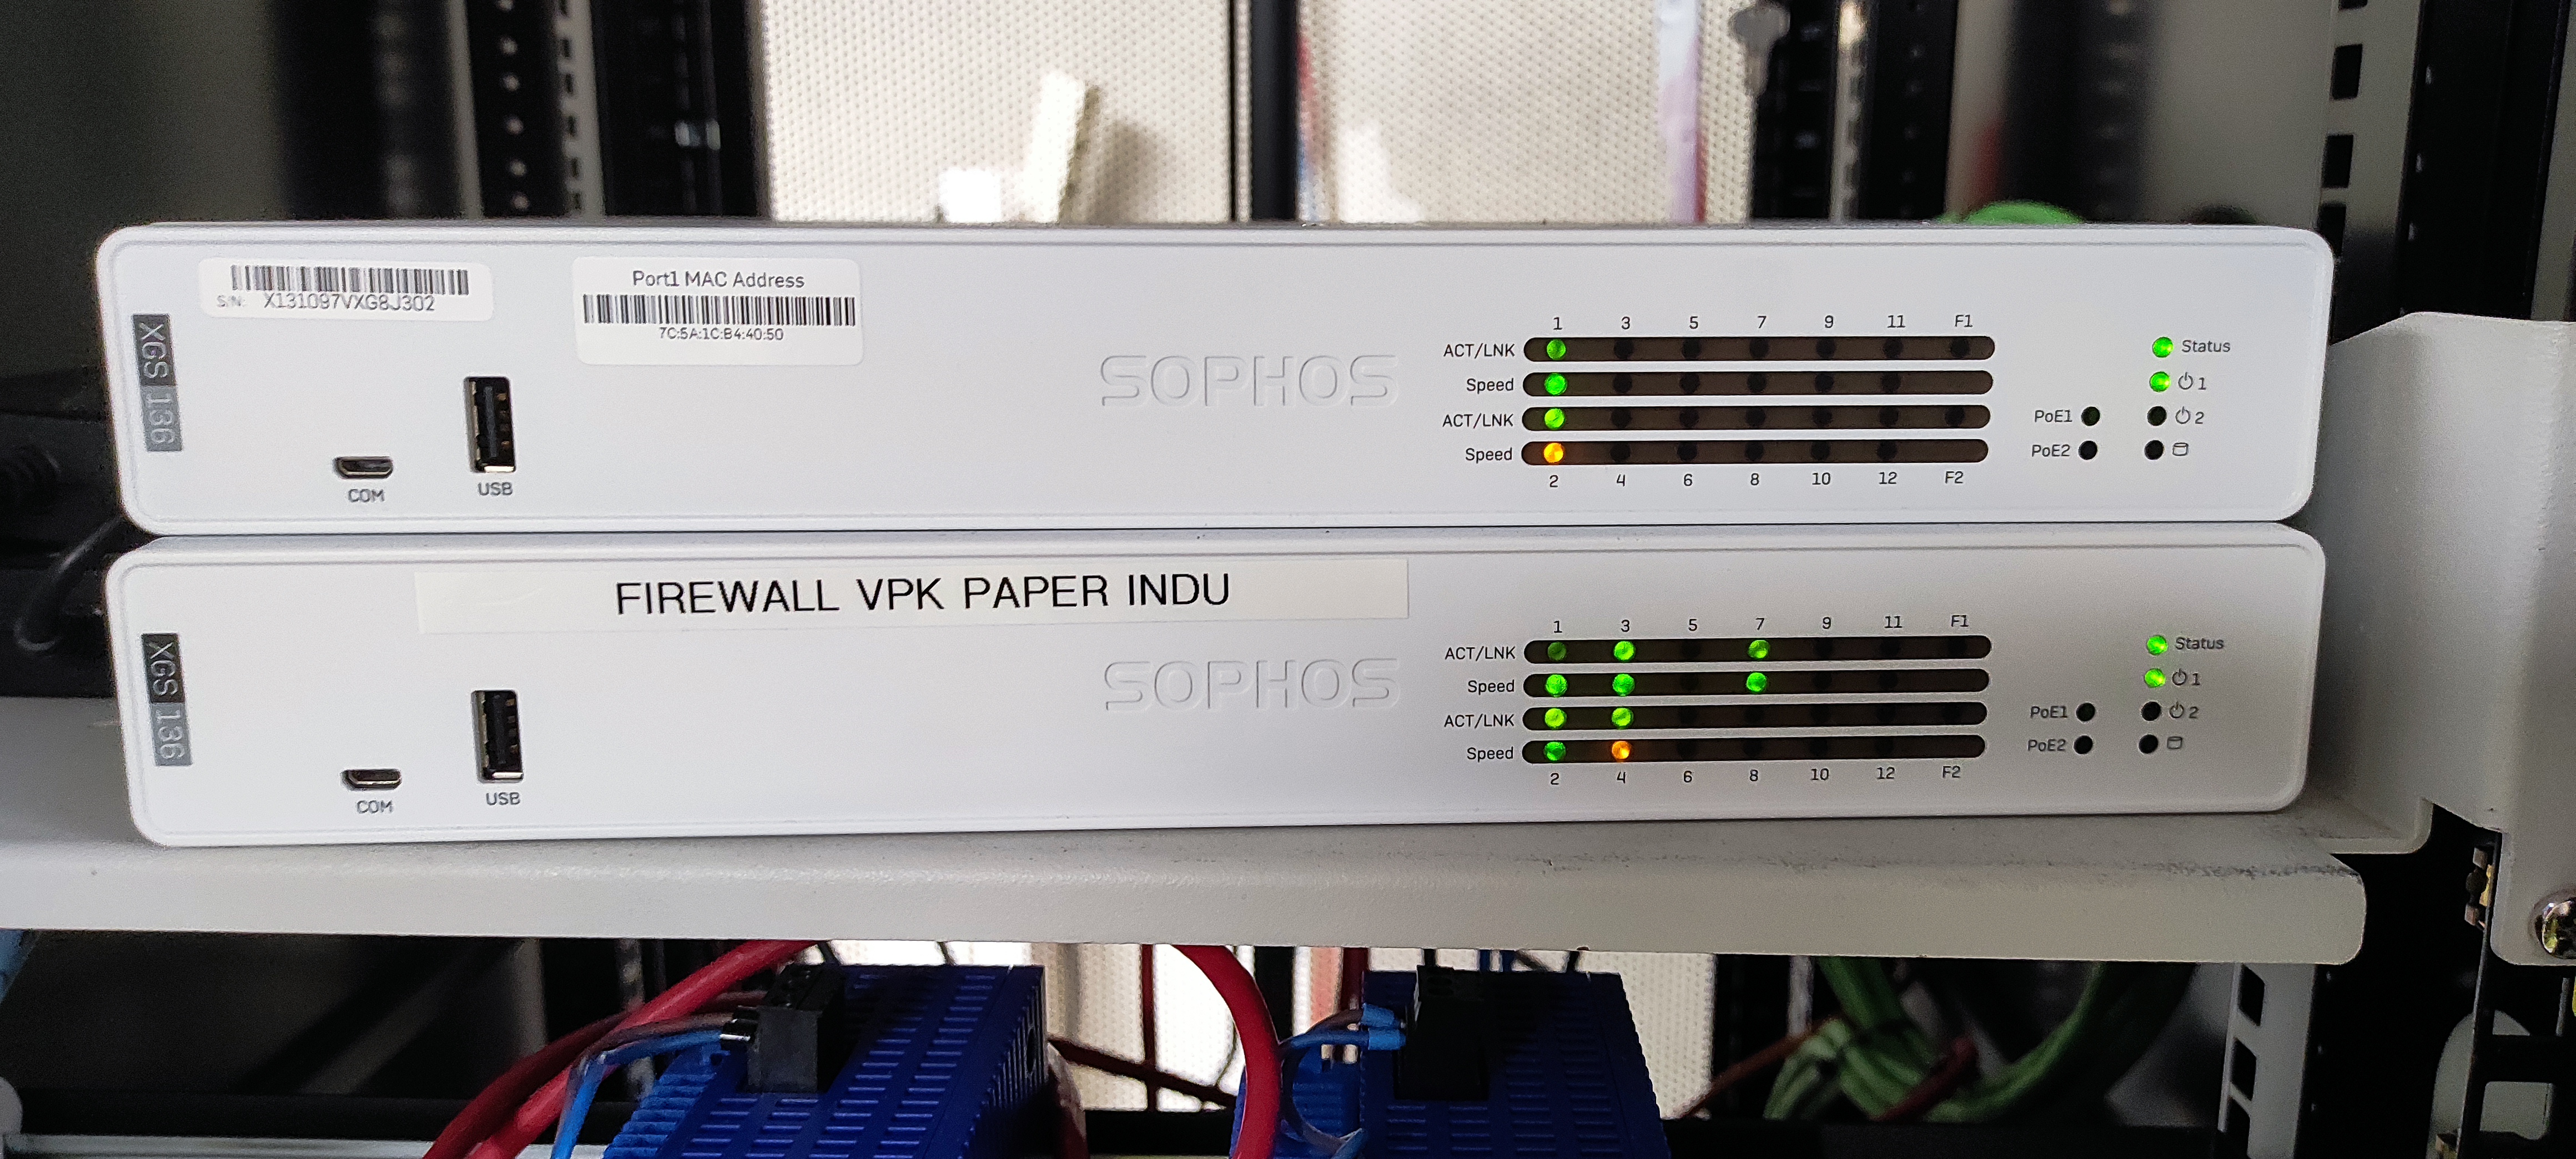
\includegraphics[width=0.8\textwidth]{fotos/SophosFirewall.jpg}
    \caption[Sophos Firewall]{\label{fig:grail}De huidige Sophos firewall die gebruikt wordt op de FR16 site van VPK.}
\end{figure} 

\subsection{Problemen met het huidige OT netwerk}
Een van de grootste uitdagingen binnen het netwerk van de productiesite van Alizay is het gebrek aan documentatie over de bestaande infrastructuur. Het netwerkteam dat verantwoordelijk was voor het onderhoud van het IT- en OT-netwerk voor de overname door VPK heeft geen gedetailleerde documentatie bijgehouden over de netwerkarchitectuur. Dit maakt het beheer van het netwerk moeilijker, omdat er onvoldoende inforimatie beschikbaar is over de werking en samenstelling ervan. Zonder deze kennis wordt het uitdagend om aanpassingen door te voeren, storingen snel op te lossen en beveiligingsrisico’s effectief te beheersen.
Het OT-netwerk binnen de site van Alizay bestaat uit meerdere generaties componenten die in de loop van tientallen jaren zijn geïmplementeerd. Hierdoor is het netwerk geleidelijk uitgebreid met verschillende subnetwerken die doorheen de jaren zijn toegevoegd, vaak zonder een plan of duidelijke standaardisatie. Dit heeft geleid tot een complexe en gefragmenteerde infrastructuur, waarbij verschillende systemen en protocollen naast elkaar bestaan.
Deze gelaagde netwerkstructuur kan verschillende uitdagingen veroorzaken wanneer wordt besloten de huidige firewallregels te herzien of te optimaliseren. Op dit moment zijn er geen specifieke firewallregels die expliciet bepalen welke data uit de verschillende subnetwerken mag worden doorgelaten of geblokkeerd. Dit betekent dat het netwerk mogelijk meer verkeer toestaat dan strikt noodzakelijk is, wat een potentieel beveiligingsrisico vormt. Tegelijkertijd zorgt het ontbreken van een duidelijke segmentatie van het netwerk ervoor dat ongewenste blokkades kunnen optreden wanneer nieuwe firewallregels worden ingevoerd.
De combinatie van een verouderde netwerkinfrastructuur en het gebrek aan een goed gedefinieerd firewallbeleid kan het risico met zich mee brengen dat bepaalde subnetwerken of systemen onverwacht worden geblokkeerd bij herconfiguratie van de firewall. Dit kan ertoe leiden dat machines tijdelijk uitvallen, wat een negatieve impact heeft op de productieprocessen en de volledige supply chain. In sommige gevallen kan zelfs een kleine onderbreking in de netwerkcommunicatie ervoor zorgen dat een machine niet meer correct functioneert, waardoor productiestilstand ontstaat en de continuiteit van de productie niet gewaarborgd kan worden.

Binnen de verschillende productiesites van VPK wordt gebruikgemaakt van machines afkomstig van diverse externe leveranciers. Deze geavanceerde machines bevatten vaak een combinatie van verschillende technische componenten, zoals PLC’s, sensoren, pneumatische systemen, robotarmen en geautomatiseerde transportsystemen zoals die van Minda. 

\begin{figure}[H]
    \centering
    \includegraphics[width=0.8\textwidth]{fotos/MindaConveyorFotoBP.jpg}
    \caption[Minda Conveyor]{\label{fig:grail} Een Minda conveyor installatie die pallets met kartonnen dozen verplaatst. ©Talina Scholz}
\end{figure} 

Deze componenten zijn onderling afhankelijk en wisselen continu data uit om productieprocessen op elkaar af te stemmen. Om deze gegevensuitwisseling mogelijk te maken moet er een betrouwbaar netwerk aanwezig zijn die alle verschillende componenten met elkaar verbindt.
In de praktijk betekent dit dat fabrikanten van deze machines vaak genoodzaakt zijn om hun eigen kleine netwerken op te zetten binnen de productiesite. Dit gebeurt met behulp van netwerkcomponenten zoals switches en routers, zodat hun machines correct kunnen functioneren. Wanneer een productiesite veel verschillende machines van uiteenlopende fabrikanten bevat, ontstaat al snel een situatie waarbij een groot aantal afzonderlijke private netwerken naast elkaar bestaat. Omdat deze netwerken zelden op elkaar worden afgestemd of gestandaardiseerd, leidt dit tot een uiterst gefragmenteerde netwerkstructuur. Hierdoor wordt het uniform beheren van de netwerken op verschillende VPK-sites vrijwel onmogelijk, aangezien elke site een unieke combinatie van leveranciers, machines en netwerktopologieën bevat.
Daarnaast vereisen veel fabrikanten een externe verbinding met hun machines om op afstand onderhoud te kunnen uitvoeren, real-time monitoring mogelijk te maken of software-updates te installeren. Dit betekent dat er op de productiesite van Alizay op twee mogelijke manieren een connectie met het internet kan worden gerealiseerd. De eerste optie is dat de fabrikant gebruikmaakt van het bestaande bekabelde netwerk van de site, dat wordt beheerd door VPK. In dit geval moet er bij de configuratie van de firewallregels rekening mee worden gehouden dat dit verkeer niet per ongeluk wordt geblokkeerd, anders verliest de fabrikant de mogelijkheid om zijn machines op afstand te beheren.
De tweede optie is dat de fabrikant een 4G-router met een eigen SIM-kaart gebruikt, zodat er geen directe verbinding met het netwerk van VPK nodig is. Hoewel dit in sommige gevallen een veiliger alternatief lijkt, introduceert het ook uitdagingen op het gebied van toezicht en controle over externe verbindingen. Soms kan het ook zijn dat een externe fabrikant gebruik maakt van een 4G-router en een fysieke verbinding met het VPK netwerk. In feite zal de fabrikant hierdoor de firewall gaan omzeilen. Dit is een uiterst kwetsbaar fenomeen dat veel schade kan berokken aan het VPK netwerk. Omdat in feite de firewall omzeild zal worden.
Beide methoden brengen aanzienlijke beveiligingsrisico’s met zich mee. Veel van de private netwerken die door machinefabrikanten worden opgezet, voldoen niet aan de meest recente cybersecuritystandaarden. Dit betekent dat ze kwetsbaar kunnen zijn voor aanvallen van buitenaf. Indien een hacker erin slaagt toegang te krijgen tot zo’n slecht beveiligd netwerk, kan dit een potentiële ingang vormen naar het bredere IT- en OT-netwerk van de productiesite. Dit zou ernstige gevolgen kunnen hebben, zoals productieonderbrekingen, verlies van kritieke data en zelfs de manipulatie van industriële processen.




\section{SWOT Analyse}
Een SWOT-analyse is handig om een duidelijk beeld te krijgen van een situatie. Het laat zien wat goed gaat en wat beter kan. Ook helpt het om opportunities te ontdekken en mogelijke threats op tijd te zien. Door alles op een rij te zetten, worden er geen belangrijke dingen vergeten. Dit maakt het makkelijker om goede keuzes te maken. Het helpt ook om beter na te denken over wat wel en niet werkt. Met een SWOT-analyse is er meer grip op de situatie. Dit zorgt ervoor dat de kans op succes groter wordt. SWOT staat voor Strengts, Weaknesses, Opportunities en Threats. Deze vier woorden worden hieronder verder in detail besproken.


\subsection{Strengths}
\begin{itemize}
\item \texttt{\textbf{Extra laag bescherming:} Er is al een Palo Alto (PA) firewall aanwezig, wat betekent dat de Sophos firewall een extra laag van bescherming biedt. Dit is positief omdat het netwerk al enige beveiliging heeft, en de extra firewall kan helpen om de beveiliging verder te versterken.}

\item \texttt{\textbf{De setup werkt, ook al is hij niet optimaal:} De huidige netwerkconfiguratie werkt wel, ook al is hij niet perfect. Dit betekent dat er geen grote storingen of onderbrekingen zijn, maar er is nog ruimte voor verbetering.}


\end{itemize}

\subsection{Weaknesses}

\begin{itemize}
\item \texttt{\textbf{Complexiteit door de Sophos firewall:} De Sophos firewall maakt het netwerkbeheer onnodig complex. Deze firewall voegt weinig extra waarde toe, maar maakt troubleshooting en het algemene beheer moeilijker. Het zou efficiënter zijn om een uniformere oplossing te hebben die makkelijk centraal te beheren is zoals een Palo Alto firewall.}

\item \texttt{\textbf{Problemen met switches en netwerkinfrastructuur:} Er zijn loops in het netwerk, unmanaged switches die fysiek niet bereikbaar zijn voor VPK, en oude HP switches die verouderd zijn. Deze zaken maken het netwerk moeilijker te beheren en kunnen leiden tot onverwachte storingen.}

\item \texttt{\textbf{Gebrek aan documentatie:} Het netwerk is slecht gedocumenteerd en niemand binnen het OT/IT team van Alizay kent de volledige netwerktopologie. Dit maakt het lastig om het netwerk te beheren, te troubleshooten of wijzigingen door te voeren zonder risico’s.}

\item \texttt{\textbf{Slechte firewallconfiguratie:} De huidige configuratie van de Sophos firewall is niet optimaal. Er zijn onnodige statische routes en ineffectieve firewallregels, wat zorgt voor extra complexiteit en mogelijk ook kwetsbaarheden in de beveiliging.}

\item \texttt{\textbf{Verouderde switches:} De HP switches die al sinds 2002 in gebruik zijn, hebben geen updates meer ontvangen. Dit maakt ze kwetsbaar voor beveiligingsrisico’s en zorgt ervoor dat ze niet optimaal functioneren. Ook zal hun ouderdom er voor zorgen dat er een grotere kans is op het falen van één of meerdere van hun onderdelen. Hierdoor is de kans dat er een outage is van één van deze devices een pak groter. }
\end{itemize}
    
\subsection{Opportunities}

\begin{itemize}
\item \texttt{\textbf{Uniformiteit creëren door de Sophos firewall te verwijderen:} Door de Sophos firewall te verwijderen, kan het netwerk binnen alle VPK-sites op dezelfde manier worden ingericht. Dit maakt het beheer veel eenvoudiger en efficiënter, doordat er één gestandaardiseerde opstelling is.}

\item \texttt{\textbf{Vervangen van oude switches:} De verouderde HP en Hirschmann switches kunnen worden vervangen door modernere en efficiëntere modellen van Hirschmann of Cisco. Dit verbetert de prestaties van het netwerk en maakt het veiliger in het geheel.}

\item \texttt{\textbf{Netwerkinfrastructuur documenteren:} Door de huidige opstelling te wijzigen is er een kans om de nieuwe netwerkstructuur goed te documenteren, wat het beheer en de troubleshooting in de toekomst veel gemakkelijker maakt.}

\item \texttt{\textbf{Vermijden van cyberdreigingen:} Door oude apparatuur en slechte configuraties te vervangen, wordt de kans op cyberaanvallen en netwerkuitval aanzienlijk verkleind. Dit verhoogt de algemene beveiliging van het netwerk.}

\item \texttt{\textbf{Segmentatie toepassen:} Er is de mogelijkheid om de netwerksegmentatie correct toe te passen, wat de beveiliging en efficiëntie van het netwerk verder kan verbeteren. Dit zorgt ervoor dat verschillende delen van het netwerk beter beschermd worden tegen dreigingen van buitenaf.}

\end{itemize}


\subsection{Threats}

\begin{itemize}
\item \texttt{\textbf{Verwijdering van de Sophos firewall kan problemen veroorzaken:} Omdat de Sophos firewall diep verweven is in het netwerk, kan het verwijderen ervan onverwachte problemen veroorzaken. Het netwerk kan niet direct goed functioneren zonder aanpassingen, wat risico’s voor de stabiliteit met zich meebrengt.}

\item \texttt{\textbf{Onbekende impact bij het verwijderen van een firewall:} Aangezien het netwerk niet goed gedocumenteerd is, kan het verwijderen van de firewall invloed hebben op onontdekte delen van het netwerk. Dit kan leiden tot onverwachte onderbrekingen of storingen.}

\item \texttt{\textbf{Externe partners kunnen beïnvloed worden:} Er zijn veel externe partners die met het netwerk verbonden zijn, zoals S2I, Evrest, en Valmet. Aanpassingen in het netwerk kunnen gevolgen hebben voor hun apparaten en systemen. Het is dus belangrijk om goed overleg te voeren met deze leveranciers om problemen te voorkomen.}

\item \texttt{\textbf{Moeilijkheden bij storing:} Als er een probleem is met netwerk apparatuur (zoals switches of routers), kan het voor het IT team van VPK heel lastig zijn om de oorzaak van het probleem snel te vinden. Dit kan leiden tot lange downtime en verstoringen in de productie.}
\end{itemize}


\section{RASCI Analyse}

Volgens \textcite{Epam2024} is RASCI een raamwerk dat specifieke rollen en verantwoordelijkheden toekent aan belanghebbenden die betrokken zijn bij een project of proces. Zie het als een routekaart die iedereen naar een gezamenlijk doel leidt zonder verwarring of vertraging. 
De verschillende letters van RASCI staan voor een bepaald woord dat een bepaalde rol samenvat.

\begin{itemize}
    \item \texttt{\textbf{Responsible:} De rol die de taak effectief uitvoert. Deze persoon of groep is de drijvende kracht achter de uitvoering van de taak. }
    \item \texttt{\textbf{Accountable:} De eindverantwoordelijke voor de taak. Deze rol draagt de verantwoordelijkheid voor het uiteindelijke succes of falen van de taak. }
    \item \texttt{\textbf{Supportive:} Een rol die ondersteuning biedt aan de 'Responsible' bij het uitvoeren van de taak. }
    \item \texttt{\textbf{Consulted:} Een persoon of rol die waardevolle input levert. Zij worden geraadpleegd voor advies en meedenken bij belangrijke beslissingen.}
    \item \texttt{\textbf{Informed:} De rol die op de hoogte wordt gehouden van beslissingen of acties die binnen de taak plaatsvinden.}
\end{itemize}

\subsection{Opbouw van de RASCI Matrix.}
Volgens \textcite{Cabanillas2011} is een RASCI-matrix is opgebouwd uit twee assen: op de horizontale as worden de verschillende rollen binnen het project weergegeven, terwijl de verticale as de diverse taken toont. In elk vakje van de matrix wordt met een enkele letter aangeduid welke rol welke verantwoordelijkheid opneemt voor een bepaalde taak. Zo staat bijvoorbeeld de letter 'R' voor "Responsible. Wanneer bijvoorbeeld de letter 'R' in een bepaald vakje voorkomt, betekent dit dat de overeenkomstige rol op de horizontale as Responsable is voor de taak op de verticale as. \autocite{Cabanillas2011}

\subsection{Verschillende taken binnen deze RASCI matrix}
\textbf{Inventarisatie van bestaand OT netwerk.}
\begin{itemize}[label=\textbullet]
    \item Deze taak omvat het in kaart brengen van alle apparaten binnen het OT-netwerk van FR16. Van elk toestel worden relevante gegevens geregistreerd, zoals het MAC-adres, IP-adres, merk, type en andere nuttige informatie.  
\end{itemize}

\textbf{Onderhouden documentatie van het OT netwerk.}
\begin{itemize}[label=\textbullet]
    \item Wanneer er wijzigingen plaatsvinden binnen het netwerk (zoals het toevoegen of verwijderen van apparaten) wordt de inventarisatie hierop aangepast. Het doel is om steeds te beschikken over een actueel netwerkplan van het OT netwerk, zodat de documentatie up-to-date blijft. 
\end{itemize}

\textbf{1st line support bieden.}
\begin{itemize}[label=\textbullet]
    \item  First-line support betreft het bieden van eerste hulp bij technische problemen of meldingen. De verantwoordelijke persoon is het eerste aanspreekpunt en probeert de meldingen zo snel en efficiënt mogelijk op te lossen, of indien nodig door te verwijzen naar een volgende ondersteuningslijn.
\end{itemize}

\textbf{Beheren van netwerkkasten externe leverancier}
\begin{itemize}[label=\textbullet]
    \item Binnen de OT-omgeving bevinden zich meerdere netwerkkasten met apparatuur van externe leveranciers, waaronder switches, routers en VPN-routers. Deze componenten zijn essentieel voor de werking van de productie-installaties. 
\end{itemize}

\textbf{Beheren van fysieke componenten binnen het OT netwerk.}
\begin{itemize}[label=\textbullet]
    \item Deze taak richt zich op het beheer van industriële hardware binnen het OT-netwerk, zoals industriële switches, PLC’s, SCADA-systemen, sensoren, en andere verbonden componenten die een directe rol spelen in de operationele processen.
\end{itemize}


\textbf{Beheren van fysieke componenten binnen het IT netwerk.}
\begin{itemize}[label=\textbullet]
    \item De fysieke componenten waar men het hier over heeft zullen voornamelijk bestaan uit: switches, routers, firewalls, servers, bekabeling, …
\end{itemize}

\textbf{Onderhouden OT firewall.}
\begin{itemize}[label=\textbullet]
    \item Binnen de huidige OT opstelling van FR16 is er een Sophos firewall aanwezig. Deze firewall wordt enkel gebruik binnen het OT netwerk. Daarom is het OT team verantwoordelijk voor het beheer van deze firewall.
\end{itemize}



\begin{figure}[H]
    \centering
    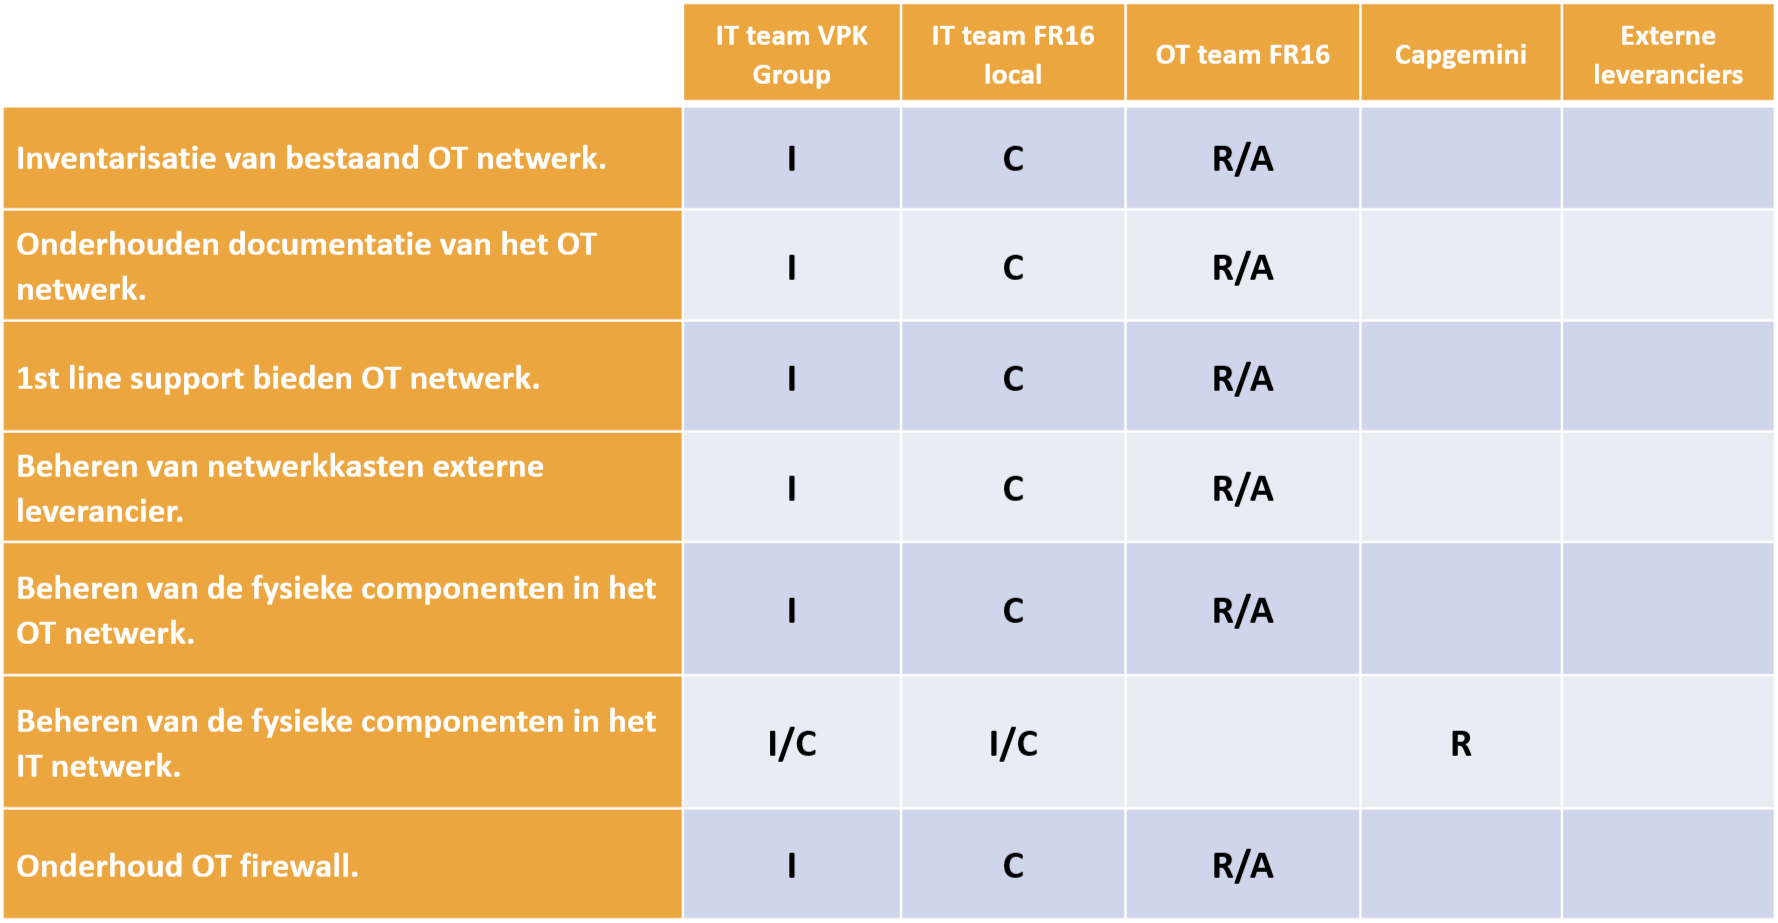
\includegraphics[width=1\textwidth]{fotos/Rasci_AS-IS.png}
    \caption[Foto Rasci AS-IS]{\label{fig:grail}Rasci tabel van de huidige toestand in FR16.}
\end{figure} 

\begin{figure}[H]
    \centering
    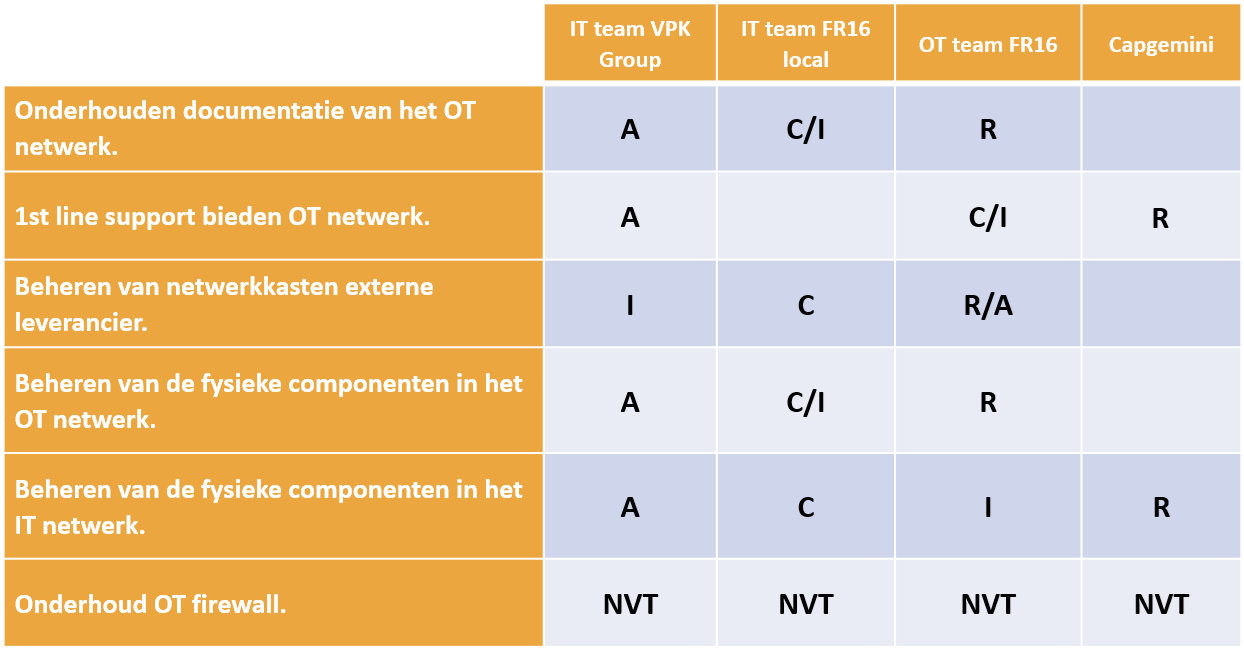
\includegraphics[width=1\textwidth]{fotos/Rasci_TO-BE.png}
    \caption[Foto Rasci TO-BE]{\label{fig:grail}Rasci tabel voor de toekomstige opstelling in FR16.}
\end{figure} 



\chapter{Configuratie van de firewall opstelling}
\label{ch:configFW}

Op basis van de verzamelde info en de huidige problemen op de productiesite van Alizay, lijkt het logisch om te kiezen voor één soort firewall die goed past bij de bestaande infrastructuur en kennis binnen VPK. Een overstap naar een Palo Alto firewall heeft op dat vlak verschillende voordelen.

Met deze oplossing kan het beheer van alle firewalls binnen VPK op één plek gebeuren. Dat maakt het dagelijkse werk minder ingewikkeld. Ook gebruiken andere VPK-sites al Palo Alto, wat zorgt voor meer eenheid. Zo kan er beter gebruik gemaakt worden van bestaande kennis, werkwijzen en tools. Dit zorgt voor een veiligere en efficiëntere werking van zowel IT- als OT-netwerken. Tegelijk verkleint het de kans op fouten of verkeerde instellingen.

Doordat Palo Alto al op meerdere plaatsen binnen VPK gebruikt wordt, kan het netwerkteam sneller reageren bij problemen of aanpassingen doen zonder hulp van buitenaf nodig te hebben. Aangezien het huidige OT-netwerk vrij complex is, is het ook belangrijk dat de firewall goede ondersteuning biedt voor het opdelen van het netwerk, het opvolgen van verkeer en het beheren van wie toegang heeft tot wat.

Daarom lijkt het logisch om de Sophos firewall te verwijderen uit het netwerk, en enkel gebruik te maken van een Palo Alto firewall pair.

\newpage

\section{Beste High Availability settings voor de Palo Alto firewalls van FR16.}


High Availability (HA) is een functie die verschillende netwerk apparatuur vendors aanbieden, deze functie zorgt ervoor dat de downtime geminimaliseerd wordt door het gebruiken van meerdere entiteiten van dezelfde appartuur. Vaak zal er gebruik worden gemaakt van twee apparaten die dan op verschillende mogelijke manieren geconfigureerd kunnen worden. Twee populaire manieren om deze apparaten te configurenen zijn Active/Active of Active/Passive. De termen Active en Passive slaan hier op de staat van het apparaat. Active betekend dat dit apparaat wel degelijk bepaalde netwerk functies op zich zal nemen en dus actief zal meerwerken om bepaalde data te verwerken. Passive betekend dat het apparaat niet actief data zal verwerken, en zich dus in een soort van rust stand bevindt.

\subsection{Active/Active firewall opstelling}
Bij een Active/Active opstelling verwerken beide apparaten actief data. In dit geval zullen beide firewalls gelijktijdig verkeer filteren op basis van vooraf gedefinieerde firewallregels. Hoewel dit in sommige situaties voordelen kan bieden, is deze opstelling in onze omgeving minder geschikt om meerdere redenen.
\newline



\begin{itemize}
    \item \textbf{Active/Active firewall pairs zijn complex om te installeren en onderhouden:}  Sessie synchronisatie tussen de firewalls kan complex worden, zeker als er gebruik wordt gemaakt van dynamische IP’s binnen het netwerk. Omdat er is besloten in bovenstaande rasci matrix dat het beheer van de OT firewall een verantwoorddelijkheid is van het OT team lijkt het niet verstandig om gebruik te maken van een complexe firewall opstelling omdat de kennis over het beheer van dit soort opstellingen minder groot is bij het OT team. 
    
    \item \textbf{Kans op asymmetrische sessies:} De kans is groter dat beide firewalls onafhankelijk data forwarden, waardoor inbound verkeer via een ander pad kan terugkeren dan outbound verkeer. Dit kan leiden tot session mismatches, met als gevolg dat data mogelijk wordt gedropt.
    
    \item \textbf{Inconsistentie met andere sites:}  Alle andere VPK-sites met een Palo Alto firewall-pair gebruiken een Active/Passive-opstelling. Een Active/Active-configuratie binnen FR16 zou de uniformiteit van de netwerkarchitectuur verstoren.

\end{itemize}

\newpage

Ook is binnen deze Active/Active opstelling de mogelijkheid om gebruik te maken van parallel processing. Dit zorgt er effectief voor dat throughput verdubbeld wordt. \autocite{Fulp2006} Voor onze use case is dit echter niet relevant. De hoeveelheid data die via de Sophos firewall wordt verstuurd, is zo laag dat één Palo Alto firewall ruim voldoende capaciteit heeft om deze load zonder merkbare vertraging te verwerken. Uit een uitgebreide analyse van het netwerkverkeer op de WAN poort van de Sophos firewall, uitgevoerd over meerdere weken en op verschillende tijdstippen, blijkt dat de maximale gemeten throughput slechts 10 KBps bedroeg.


De nieuwe Palo Alto firewall (PA-440) zou een maximale throughput van 2,6 Gbps hebben en ondersteunt 200.000 gelijktijdige sessies. \autocite{PaloAltoDS2025} Dit betekent dat de beschikbare capaciteit ruimschoots volstaat en dat een Active/Active configuratie geen toegevoegde waarde biedt voor deze specifieke productiesite.

\begin{figure}[H]
    \centering
    \fbox{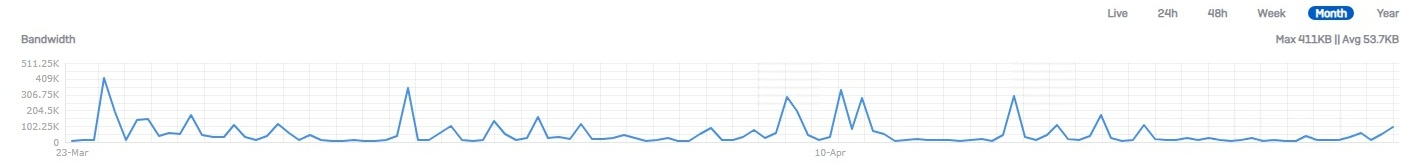
\includegraphics[scale=0.41]{fotos/SophosBandWidth.jpg}}
    \caption[Sophos firewall bandwidth graph]{\label{fig:grail}Totale bandbreedte die gebruikt wordt door de Sophos OT firewall van de productiesite van FR16}
\end{figure}




\subsection{Active/Passive firewall opstelling}

In een Active/Passive-opstelling is er slechts één firewall die gelijktijdig data verwerkt. Dit wordt mogelijk gemaakt door het configureren van HA-links. Deze links zijn cruciaal voor het waarborgen van redundantie, hoge prestaties en synchronisatie tussen firewalls in een HA-pair. Ze stellen de firewalls in staat om met elkaar te communiceren en statusinformatie te delen. Hierdoor kan de passieve firewall moeiteloos de taak van de actieve firewall overnemen bij een eventuele uitval. Zo zorgt de actieve firewall ervoor dat sessie-informatie wordt gedeeld met de passieve firewall, zodat deze altijd over de benodigde sessiegegevens beschikt in het geval van een failover. \autocite{PaloAltoHA2025} \autocite{PaloAltoHAb2025}

Verder in dit hoofdstuk zal een HA verbinding tussen twee firewalls worden geconfigureerd op basis van de behoeften van VPK en de algemene best practices.

\begin{figure}[H]
    \centering
    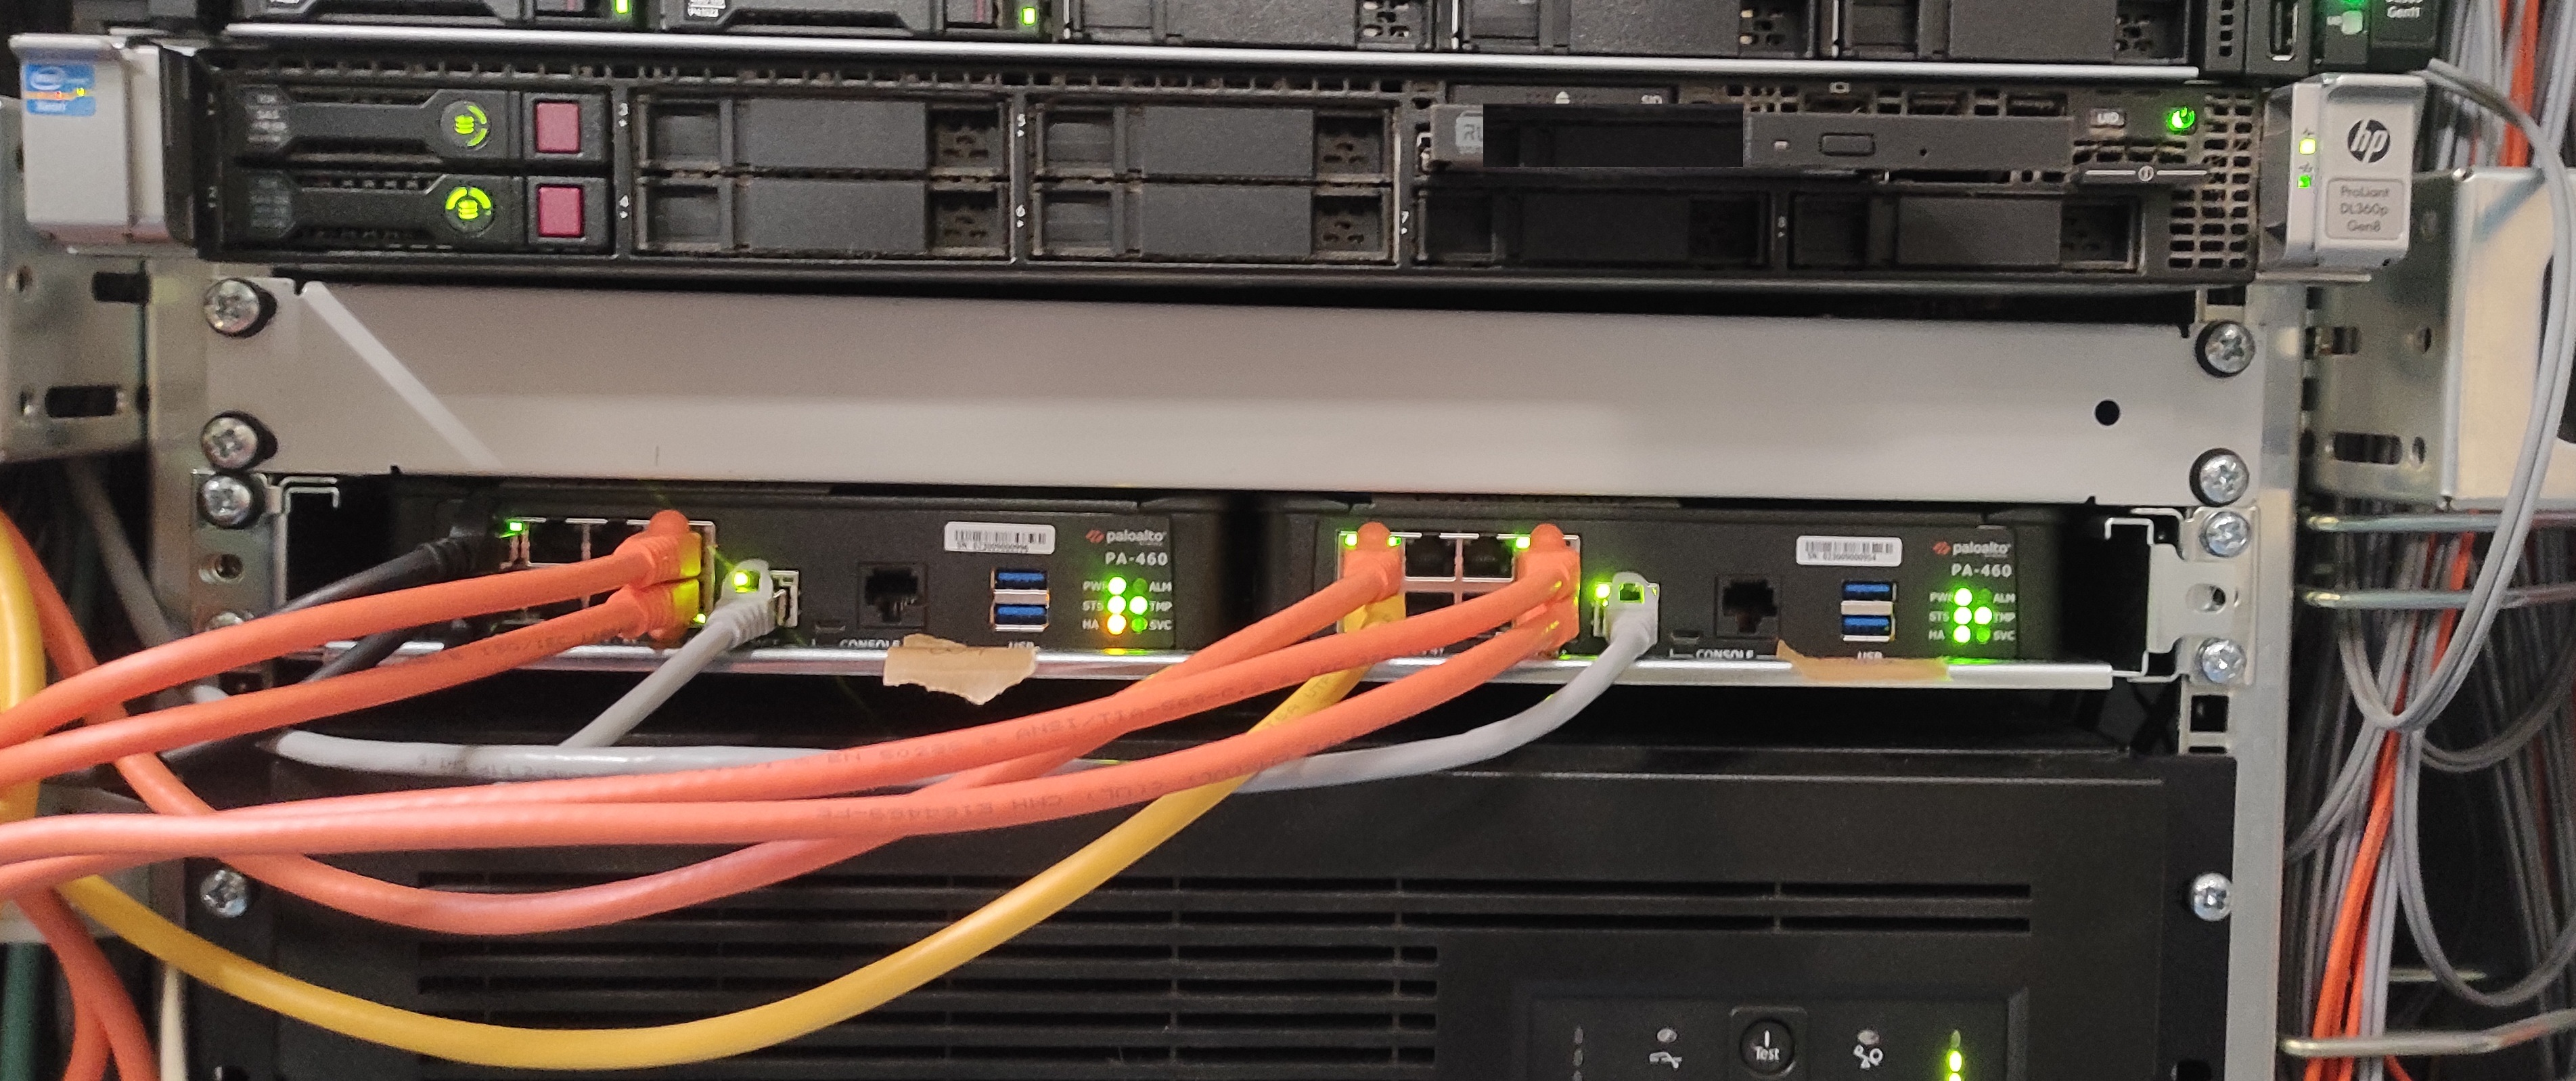
\includegraphics[width=0.8\textwidth]{fotos/PA_FirewallPairBE02.jpg}
    \caption[Palo Alto Active/Passive pair]{\label{fig:grail}Een Palo Alto Active/Passive firewall opstelling in de VPK site van Erembodegem.}
\end{figure} 



\section{Beste High Availability settings voor de Sophos firewall van FR16}

Om gebruik te kunnen maken van de HA-functies van de Sophos firewall is het noodzakelijk om twee identieke firewalls aan te schaffen. Momenteel is er echter slechts één firewall aanwezig, waardoor VPK genoodzaakt zal zijn om een tweede Sophos firewall aan te kopen om HA te kunnen implementeren. Dit proces is echter niet eenvoudig, aangezien het onduidelijk is hoe de huidige Sophos firewall is geconfigureerd. Als de twee firewalls in het HA-paar verschillende instellingen hebben, kan dit in de toekomst mogelijk problemen veroorzaken. Daarom moet er een tweede identieke firewall worden aangeschaft, en is het essentieel om een onderzoek te doen naar de huidige configuratie van de Sophos firewall.



\section{Verzamelen en verwerken van Logs}

\subsection{Logs via Palo Alto}
De Palo Alto firewalls die zich op andere locaties bevinden, verzamelen loggegevens van netwerkverkeer en systeemactiviteiten. Deze logs worden automatisch doorgestuurd naar een centrale server waarop Microsoft Sentinel draait. Microsoft Sentinel is een cloudgebaseerde SIEM-oplossing van Microsoft. SIEM staat voor Security Information and Event Management.
Een SIEM systeem verzameld loggegevens uit verschillende bronnen, zoals firewalls, servers, toepassingen en andere netwerkapparaten. Die gegevens worden vervolgens geanalyseerd. Als er iets gebeurt dat afwijkt van het normale gedrag, kan Sentinel dit detecteren in realtime. Het systeem kan daarna automatisch meldingen sturen of zelfs actie ondernemen, zoals het blokkeren van een IP-adres of het starten van een onderzoek. Zo helpt Sentinel bij het vroegtijdig opsporen van cyberdreigingen en bij het verbeteren van de beveiliging van het netwerk.


Naast Microsoft Sentinel worden de verzamelde loggegevens ook doorgestuurd naar de Zabbix monitoringserver. Zabbix is een open-source monitoringtool die gebruikt wordt om IT-infrastructuur te bewaken. Dit omvat onder andere fysieke servers, virtuele machines, netwerksystemen en cloudtoepassingen.
Zabbix verzamelt allerlei metrics zoals CPU-belasting, geheugengebruik, schijfruimte, netwerkactiviteit, enzovoort. Deze informatie wordt weergegeven in een overzichtelijk dashboard dat je via een webinterface kan bekijken. Zo kan er in één oogopslag gezien worden of er problemen zijn met een bepaald systeem of apparaat.
Zabbix maakt het ook mogelijk om alerts te versturen wanneer bepaalde drempels worden overschreden, bijvoorbeeld als de CPU belasting te hoog is of als een server niet meer reageert. Op die manier kunnen problemen snel worden gedetecteerd en opgelost, voordat ze ernstige gevolgen hebben.

\begin{figure}[H]
    \centering
    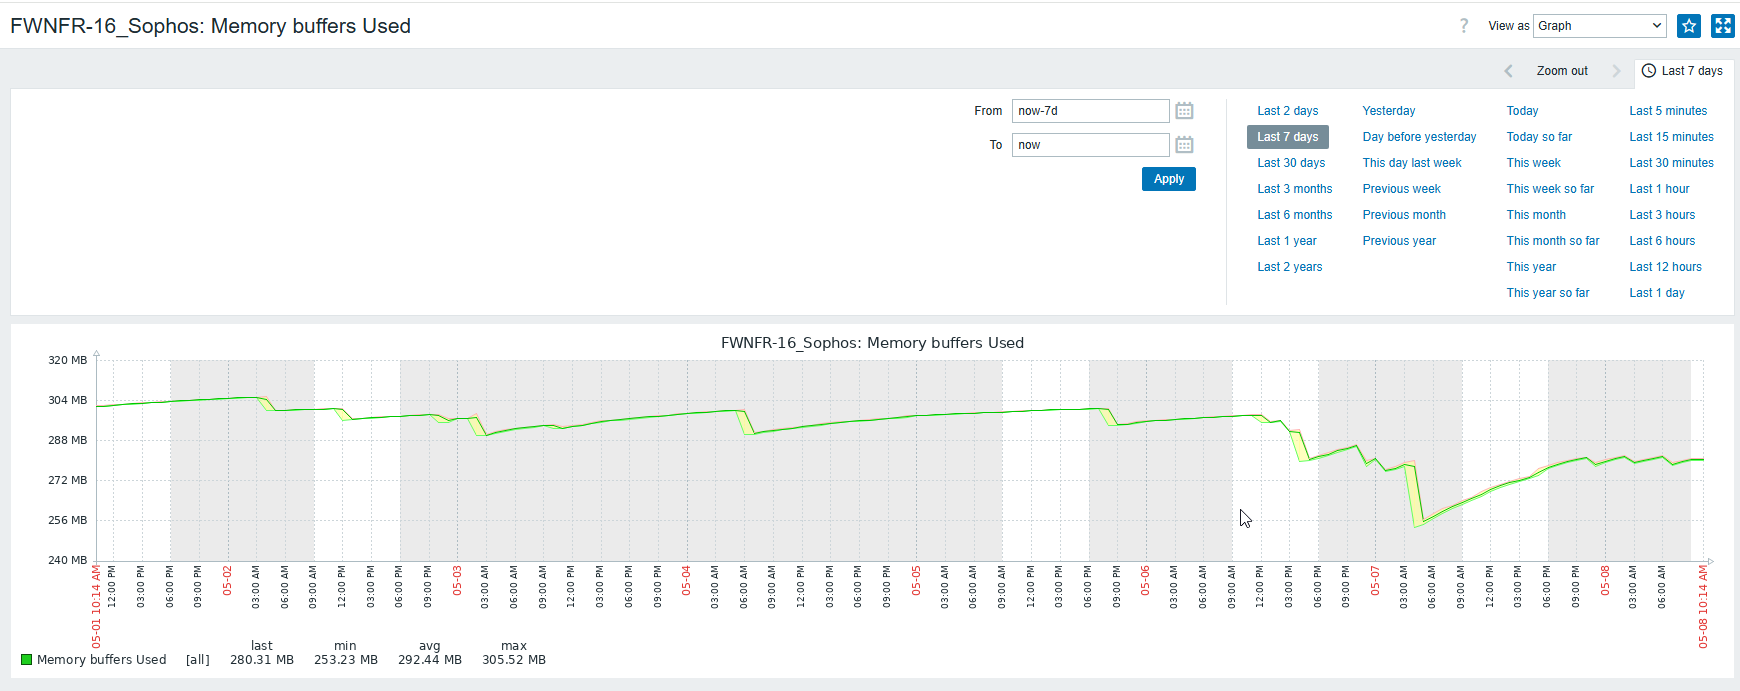
\includegraphics[width=0.9\textwidth]{fotos/SophosZabbix.png}
    \caption[Sophos Memory Buffer in Zabbix]{\label{fig:grail}Een grafiek uit Zabbix die het geheugengebruik van de memory buffers van de Sophos firewall in Mega Bytes weergeeft.}
\end{figure} 


\subsection{Logs via Sophos}
Tot voor kort werden er op de Sophos firewall geen loggegevens verzameld. Hierdoor was er weinig zicht op wat er zich precies afspeelde binnen het netwerkverkeer dat via deze firewall liep. Als onderdeel van mijn bachelorproef heb ik ervoor gezorgd dat de firewall nu wel logs verzamelt en dat deze op een correcte en veilige manier worden doorgestuurd naar de nodige servers die de data analyseren en verwerken.
De loggegevens worden via het syslog-protocol doorgestuurd naar twee verschillende servers: enerzijds de Zabbix monitoringserver en anderzijds de Microsoft Sentinel server. Deze syslog-berichten bevatten nuttige informatie, zoals de actuele firewallregels, de heartbeat van het systeem en verschillende systeemgebeurtenissen.
Omdat er op het FR16-netwerk tot nu toe nauwelijks of geen monitoring aanwezig was, is deze wijziging van groot belang. Dankzij deze aanpassing kunnen problemen sneller worden opgemerkt. In het geval van downtime of een mogelijke cyberdreiging kan er sneller worden ingegrepen, wat uiteindelijk helpt om schade of downtime te beperken.



\section{Configuratie van HA op een Palo Alto Firewall}

\textbf{Mode}
    \begin{itemize}[label=\textbullet]
        \item Zoals eerder in dit hoofdstuk besproken is zal er bij de configuratie van een Palo Alto firewall pair binnen een VPK site gebruik worden gemaakt van een Active/Passive opstelling. Hierbij zal er steeds slechts één firewall tegelijk actief zijn.
    \end{itemize}



\textbf{Enable Config Sync}
    \begin{itemize}[label=\textbullet]
        \item Configuration synchronization is een setting binnen Palo Alto HA firewall pairs. Waarbij een groot aantal settings automatisch worden gesyncroniseerd tussen devices. Om conflicten in configuraties te vermijden is het steeds aangeraden om configuraties steeds op de Active firewall uit te voeren en te wachten tot de Passive firewall gesynced is. Een aantal settings die niet worden gesynchroniseerd zijn: content updates, HA settings, mgmt interface settings, \ldots 
    \end{itemize}



\textbf{Passive Link state}
    \begin{itemize}[label=\textbullet]
        \item Deze settings zal bepalen in welke status alle data interfaces van een Passive firewall zullen worden geplaatst. Bij het gebruiken van de `shutdown` modus zullen alle data interfaces op de passive firewall in een `down` state worden geplaatst. Naast deze modus is er ook de `auto` modus. Bij deze modus zal alle data interfaces op `up` laten staan, maar dropped alle packets die over deze interfaces zouden passeren. Echter zou dit er voor kunnen zorgen dat switches nog steeds data packets zouden versturen over deze schijnbare `up` interfaces. Dit probleem samen met de algemene beste hardening cybersecurity practices om alle poorten die niet gebruikt worden op `down` te zetten zorgt ervoor dat VPK gebruik zal maken van de `shutdown` modus op beide firewalls.
    \end{itemize}



\textbf{Monitor fail hold down time}
    \begin{itemize}[label=\textbullet]
        \item De ``monitor fail hold down time'' is een vooraf ingestelde timer om onnodige failover te voorkomen. Nadat één van de links down gaat zal het process geen nieuwe failover toestaan als het ziet dat er binnen de tijdslimiet van één minuut de interface terug `up` is. Mocht de link toch langer dan één minuut down zijn zal er toch een failover gebeuren. Binnen iedere andere firewall op een VPK site wordt deze zelfde timer gebruikt. Daarom is er in het belang van uniformiteit gekozen om ook op deze site de timer in te stellen op één minuut.
    \end{itemize}



\textbf{Device Priority}
    \begin{itemize}[label=\textbullet]
        \item Deze settings zal bepalen welke prioriteit een bepaalde firewall heeft binnen een HA firewall pair. Een hogere waarde betekent direct ook een hogere prioriteit. Echter is dit enkel nuttig als men gebruik maakt van preemption. Maar aangezien preemption uit staat op deze firewalls zal deze priority waarde dus geen nut hebben.
    \end{itemize}



\textbf{Preemptive}
    \begin{itemize}[label=\textbullet]
        \item Deze setting zal er voor zorgen dat de firewall met een hogere prioriteit in staat is om terug Active te worden nadat er een failover is gebeurd. Echter heeft VPK gekozen om deze setting niet in te schakelen bij alle firewalls op alle VPK sites.
    \end{itemize}



\textbf{Hearbeat backup}
    \begin{itemize}[label=\textbullet]
        \item Deze optie zorgt ervoor dat er een backup is om de hearbeat berichten van de apparaten op te sturen via de management interfaces van de firewall. Deze berichten zullen standaard over de HA1 en HA2 link worden verstuurd. Aangezien er twee rechtstreekse linken zijn tussen de twee firewalls in het HA pair is het dus niet meer nodig om deze optie aan te zetten.
    \end{itemize}


\begin{figure}[H]
    \centering
    \fbox{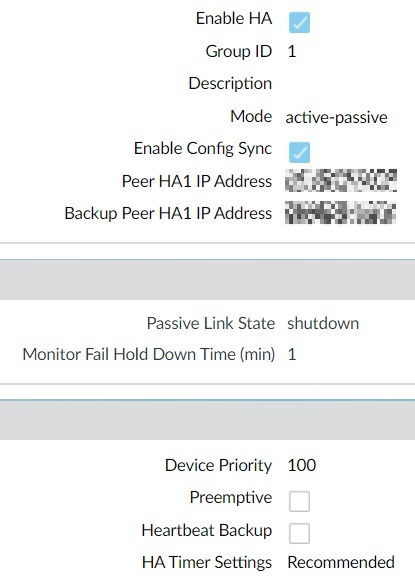
\includegraphics[scale=0.666]{fotos/PA_HASettings.jpg}}
    \caption[PA High Availability settings]{\label{fig:grail}GUI (Graphical User Interface) interface om de settings om de configuratie van High Availability op een PA firewall aan te passen.}
\end{figure}


\section{Netwerksegmentatie aan de hand van VLAN’s}

Netwerksegmentatie met VLAN’s (Virtual Local Area Networks) is nog steeds een erg goede manier om verschillende delen van een netwerk virtueel van elkaar te scheiden. Daarom lijkt het een slim idee om deze techniek ook toe te passen op het VPK-netwerk.

Concreet kan ervoor gekozen worden om de apparaten die binnen het IT/OT netwerk actief zijn onder te verdelen in verschillende groepen. Zo worden deze groepen van elkaar afgescheiden en is communicatie tussen hen standaard niet meer mogelijk. Uiteraard kunnen we nog steeds toestaan dat bepaalde groepen met elkaar praten via firewallregels op de Palo Alto firewall.

Het belangrijkste doel hiervan is simpel: als een aanvaller erin slaagt om toegang te krijgen tot één apparaat, dan krijgt hij niet meteen toegang tot het volledige netwerk, maar blijft hij beperkt tot het VLAN waarin dat toestel zich bevindt.

Om het allemaal overzichtelijk te houden, is het ook aangeraden om de VLAN’s te koppelen aan specifieke IP-ranges. Zo is het makkelijker om snel te zien in welk VLAN een bepaald toestel zit.

\subsection*{Voorbeeld VLAN-indeling}

\begin{table}[h!]
    \centering
    \begin{tabular}{|l|l|c|l|l|c|}
        \hline
        \textbf{DHCP} & \textbf{Usable range} & \textbf{VLAN} & \textbf{Name} & \textbf{Gateway} & \textbf{Mask} \\
        \hline
        10.x.2.0 & 10.x.2.1 -- 10.x.2.240 & 2 & AP mgmt & 10.x.2.254 & /24 \\
        10.x.4.0 & 10.x.4.1 -- 10.x.4.240 & 4 & Switch mgmt & 10.x.4.254 & /24 \\
        10.x.8.0 & 10.x.8.1 -- 10.x.8.240 & 8 & Server & 10.x.8.254 & /24 \\
        10.x.9.0 & 10.x.9.1 -- 10.x.9.240 & 9 & RF\_Corporate & 10.x.9.254 & /24 \\
        \hline
    \end{tabular}
    \caption{Een aantal gebruikte VLAN's binnen het VPK netwerk en bijhorende IP-ranges}
\end{table}

Uit het bovenstaande voorbeeld kan je afleiden dat er gekozen is om binnen VPK VLAN 8 te gebruiken voor alle servers binnen het netwerk. Zo weten we meteen dat een toestel met een IP-adres in de vorm van x.x.8.x een server is. Deze manier van werken brengt verschillende voordelen met zich mee:

\begin{itemize}
    \item \textbf{Overzichtelijkheid:} Door vaste IP-ranges per VLAN te gebruiken, is het snel duidelijk tot welke categorie een toestel behoort. Dit maakt het beheer en de troubleshooting veel eenvoudiger.
    \item \textbf{Beter beveiligd:} Apparaten die tot dezelfde functie horen (zoals servers) zitten samen in één VLAN. Dit beperkt de schade als er iets misloopt.
    \item \textbf{Efficiëntere netwerkconfiguratie:} Firewalls en andere beveiligingsregels kunnen veel gerichter ingesteld worden.
    \item \textbf{Makkelijker uitbreidbaar:} Je weet meteen in welke IP-range nieuwe toestellen moeten komen.
    \item \textbf{Snellere probleemoplossing:} Het IP-adres geeft snel inzicht in het type toestel en het netwerksegment.
    \item \textbf{Uniformiteit over verschillende sites:} Eén consistente VLAN-structuur vergemakkelijkt het beheer over meerdere locaties.
\end{itemize}

In het netwerk kan er ook voor gekozen worden om elke externe leverancier in een aparte VLAN onder te brengen. Bijvoorbeeld: Minda, Ducker, Bobst en Gopfert hebben elk hun eigen VLAN en aparte IP-range. Dit biedt heel wat voordelen:

\begin{itemize}
    \item \textbf{Verhoogde veiligheid:} Problemen blijven beperkt tot de VLAN van de leverancier.
    \item \textbf{Gerichte toegangscontrole:} Per VLAN kan je precies bepalen welke toegang een leverancier krijgt.
    \item \textbf{Compliance:} Helpt bij het voldoen aan interne en externe auditvereisten.
\end{itemize}

\section{Verschillende fases bij het deployen van firewall rules}

Bij de implementatie van de nieuwe firewalls wordt er gekozen om de firewallregels gefaseerd uit te rollen. Dit betekent dat niet alle regels in één keer actief worden, maar dat het netwerk stap voor stap verder wordt afgeschermd. Door steeds specifiekere regels in te voeren.

\subsection*{Voordelen van gefaseerde implementatie}

\begin{itemize}
    \item \textbf{Minder risico:} Fouten worden sneller opgemerkt en bijgestuurd.
    \item \textbf{Eenvoudigere probleemoplossing:} Door de gefaseerde aanpak kan men sneller de oorzaak van problemen vinden.
    \item \textbf{Beperkte OT documentatie:} Onverwachte sessies kunnen zonder onmiddellijke blokkering worden geanalyseerd.
    \item \textbf{Minimale impact op bedrijfsprocessen:} Kritieke toepassingen blijven beschikbaar tot in de laatste fase.
\end{itemize}







% Voeg hier je eigen hoofdstukken toe die de ``corpus'' van je bachelorproef
% vormen. De structuur en titels hangen af van je eigen onderzoek. Je kan bv.
% elke fase in je onderzoek in een apart hoofdstuk bespreken.

%\input{...}
%\input{...}
%...

%%=============================================================================
%% Conclusie
%%=============================================================================

\chapter{Conclusie}%
\label{ch:conclusie}

% TODO: Trek een duidelijke conclusie, in de vorm van een antwoord op de
% onderzoeksvra(a)g(en). Wat was jouw bijdrage aan het onderzoeksdomein en
% hoe biedt dit meerwaarde aan het vakgebied/doelgroep? 
% Reflecteer kritisch over het resultaat. In Engelse teksten wordt deze sectie
% ``Discussion'' genoemd. Had je deze uitkomst verwacht? Zijn er zaken die nog
% niet duidelijk zijn?
% Heeft het onderzoek geleid tot nieuwe vragen die uitnodigen tot verder 
%onderzoek?

\lipsum[76-80]



%---------- Bijlagen -----------------------------------------------------------

\appendix

\chapter{Onderzoeksvoorstel}

Het onderwerp van deze bachelorproef is gebaseerd op een onderzoeksvoorstel dat vooraf werd beoordeeld door de promotor. Dat voorstel is opgenomen in deze bijlage.

%% TODO: 
%\section*{Samenvatting}

% Kopieer en plak hier de samenvatting (abstract) van je onderzoeksvoorstel.

% Verwijzing naar het bestand met de inhoud van het onderzoeksvoorstel
%---------- Inleiding ---------------------------------------------------------

% TODO: Is dit voorstel gebaseerd op een paper van Research Methods die je
% vorig jaar hebt ingediend? Heb je daarbij eventueel samengewerkt met een
% andere student?
% Zo ja, haal dan de tekst hieronder uit commentaar en pas aan.

%\paragraph{Opmerking}

% Dit voorstel is gebaseerd op het onderzoeksvoorstel dat werd geschreven in het
% kader van het vak Research Methods dat ik (vorig/dit) academiejaar heb
% uitgewerkt (met medesturent VOORNAAM NAAM als mede-auteur).
% 

\section{Inleiding}%
\label{sec:inleiding}

Waarover zal je bachelorproef gaan? Introduceer het thema en zorg dat volgende zaken zeker duidelijk aanwezig zijn:

\begin{itemize}
  \item kaderen thema
  \item de doelgroep
  \item de probleemstelling en (centrale) onderzoeksvraag
  \item de onderzoeksdoelstelling
\end{itemize}

Denk er aan: een typische bachelorproef is \textit{toegepast onderzoek}, wat betekent dat je start vanuit een concrete probleemsituatie in bedrijfscontext, een \textbf{casus}. Het is belangrijk om je onderwerp goed af te bakenen: je gaat voor die \textit{ene specifieke probleemsituatie} op zoek naar een goede oplossing, op basis van de huidige kennis in het vakgebied.

De doelgroep moet ook concreet en duidelijk zijn, dus geen algemene of vaag gedefinieerde groepen zoals \emph{bedrijven}, \emph{developers}, \emph{Vlamingen}, enz. Je richt je in elk geval op it-professionals, een bachelorproef is geen populariserende tekst. Eén specifiek bedrijf (die te maken hebben met een concrete probleemsituatie) is dus beter dan \emph{bedrijven} in het algemeen.

Formuleer duidelijk de onderzoeksvraag! De begeleiders lezen nog steeds te veel voorstellen waarin we geen onderzoeksvraag terugvinden.

Schrijf ook iets over de doelstelling. Wat zie je als het concrete eindresultaat van je onderzoek, naast de uitgeschreven scriptie? Is het een proof-of-concept, een rapport met aanbevelingen, \ldots Met welk eindresultaat kan je je bachelorproef als een succes beschouwen?

%---------- Stand van zaken ---------------------------------------------------

\section{Literatuurstudie}%
\label{sec:literatuurstudie}

Hier beschrijf je de \emph{state-of-the-art} rondom je gekozen onderzoeksdomein, d.w.z.\ een inleidende, doorlopende tekst over het onderzoeksdomein van je bachelorproef. Je steunt daarbij heel sterk op de professionele \emph{vakliteratuur}, en niet zozeer op populariserende teksten voor een breed publiek. Wat is de huidige stand van zaken in dit domein, en wat zijn nog eventuele open vragen (die misschien de aanleiding waren tot je onderzoeksvraag!)?

Je mag de titel van deze sectie ook aanpassen (literatuurstudie, stand van zaken, enz.). Zijn er al gelijkaardige onderzoeken gevoerd? Wat concluderen ze? Wat is het verschil met jouw onderzoek?

Verwijs bij elke introductie van een term of bewering over het domein naar de vakliteratuur, bijvoorbee Denk zeker goed na welke werken je refereert en waarom.

Draag zorg voor correcte literatuurverwijzingen! Een bronvermelding hoort thuis \emph{binnen} de zin waar je je op die bron baseert, dus niet er buiten! Maak meteen een verwijzing als je gebruik maakt van een bron. Doe dit dus \emph{niet} aan het einde van een lange paragraaf. Baseer nooit teveel aansluitende tekst op eenzelfde bron.

Als je informatie over bronnen verzamelt in JabRef, zorg er dan voor dat alle nodige info aanwezig is om de bron terug te vinden (zoals uitvoerig besproken in de lessen Research Methods).

% Voor literatuurverwijzingen zijn er twee belangrijke commando's:
% \autocite{KEY} => (Auteur, jaartal) Gebruik dit als de naam van de auteur
%   geen onderdeel is van de zin.
% \textcite{KEY} => Auteur (jaartal)  Gebruik dit als de auteursnaam wel een
%   functie heeft in de zin (bv. ``Uit onderzoek door Doll & Hill (1954) bleek
%   ...'')

Je mag deze sectie nog verder onderverdelen in subsecties als dit de structuur van de tekst kan verduidelijken.

%---------- Methodologie ------------------------------------------------------
\section{Methodologie}%
\label{sec:methodologie}

Hier beschrijf je hoe je van plan bent het onderzoek te voeren. Welke onderzoekstechniek ga je toepassen om elk van je onderzoeksvragen te beantwoorden? Gebruik je hiervoor literatuurstudie, interviews met belanghebbenden (bv.~voor requirements-analyse), experimenten, simulaties, vergelijkende studie, risico-analyse, PoC, \ldots?

Valt je onderwerp onder één van de typische soorten bachelorproeven die besproken zijn in de lessen Research Methods (bv.\ vergelijkende studie of risico-analyse)? Zorg er dan ook voor dat we duidelijk de verschillende stappen terug vinden die we verwachten in dit soort onderzoek!

Vermijd onderzoekstechnieken die geen objectieve, meetbare resultaten kunnen opleveren. Enquêtes, bijvoorbeeld, zijn voor een bachelorproef informatica meestal \textbf{niet geschikt}. De antwoorden zijn eerder meningen dan feiten en in de praktijk blijkt het ook bijzonder moeilijk om voldoende respondenten te vinden. Studenten die een enquête willen voeren, hebben meestal ook geen goede definitie van de populatie, waardoor ook niet kan aangetoond worden dat eventuele resultaten representatief zijn.

Uit dit onderdeel moet duidelijk naar voor komen dat je bachelorproef ook technisch voldoen\-de diepgang zal bevatten. Het zou niet kloppen als een bachelorproef informatica ook door bv.\ een student marketing zou kunnen uitgevoerd worden.

Je beschrijft ook al welke tools (hardware, software, diensten, \ldots) je denkt hiervoor te gebruiken of te ontwikkelen.

Probeer ook een tijdschatting te maken. Hoe lang zal je met elke fase van je onderzoek bezig zijn en wat zijn de concrete \emph{deliverables} in elke fase?

%---------- Verwachte resultaten ----------------------------------------------
\section{Verwacht resultaat, conclusie}%
\label{sec:verwachte_resultaten}

Hier beschrijf je welke resultaten je verwacht. Als je metingen en simulaties uitvoert, kan je hier al mock-ups maken van de grafieken samen met de verwachte conclusies. Benoem zeker al je assen en de onderdelen van de grafiek die je gaat gebruiken. Dit zorgt ervoor dat je concreet weet welk soort data je moet verzamelen en hoe je die moet meten.

Wat heeft de doelgroep van je onderzoek aan het resultaat? Op welke manier zorgt jouw bachelorproef voor een meerwaarde?

Hier beschrijf je wat je verwacht uit je onderzoek, met de motivatie waarom. Het is \textbf{niet} erg indien uit je onderzoek andere resultaten en conclusies vloeien dan dat je hier beschrijft: het is dan juist interessant om te onderzoeken waarom jouw hypothesen niet overeenkomen met de resultaten.



%%---------- Andere bijlagen --------------------------------------------------
% TODO: Voeg hier eventuele andere bijlagen toe. Bv. als je deze BP voor de
% tweede keer indient, een overzicht van de verbeteringen t.o.v. het origineel.
%\input{...}

%%---------- Backmatter, referentielijst ---------------------------------------

\backmatter{}

\setlength\bibitemsep{2pt} %% Add Some space between the bibliograpy entries
\printbibliography[heading=bibintoc]

\end{document}
